\documentclass{book}

\title{Appunti di Teoria dei segnali}
\author{Stefano Rossini}

\usepackage{bookmark}

\usepackage[italian]{babel}
\usepackage{geometry}
\geometry{a4paper, margin={2.54cm,1.9cm}}

\usepackage{hyperref}
\usepackage{tcolorbox} %for COLORED BOXES 

\usepackage{amsmath}
\usepackage{graphicx}
\graphicspath{{./immagini/}}

\usepackage{url}

\usepackage{physics}

\usepackage{amsfonts} 

\usepackage{gensymb}

\usepackage{textcomp}

\begin{document}

\maketitle

%\setcounter{chapter}{-1}
\section*{Introduzione}

 

Appunti ordinati, con approfondimenti passo-passo, del corso di Teoria dei segnali (ora Segnali Determinati e aleatori) per il corso di laurea in Ingegneria Elettronica 
presso l’Università Politecnica delle Marche. \newline
        



Le fonti degli appunti sono le seguenti: 

\begin{itemize}
    
    \item Slide del corso del prof Franco Chiaraluce Segnali Determinati E Aleatori A.A. 2024/2025
    

\end{itemize}

\begin{tcolorbox}
    Negli appunti ci saranno delle piccole appendici dentro a questi mini-paragrafi  
    su come si leggono in italiano le varie formule matematiche,  
    e lascerò link su possibili approfondimenti matematici usando le animazioni, 
    così è più facile comprendere la materia.
\end{tcolorbox}


Per le lettere greche che ci saranno nel corso, vi consiglio di visitare questo sito \\ 
\url{https://www.rapidtables.org/it/math/symbols/greek_alphabet.html} \break 
in cui è disponibile anche la pronuncia vocale delle lettere. \newline

Le figure senza l'indicazione sono presi dalle dispense del corso, 
sennò è esplicitato il link dell'immagine. \newline 

Gli appunti del corso scritti dal prof sono sufficienti per passare il corso e mi congratulo pubblicamente con il prof per essere un prof con la P maiuscola, ce ne sono veramente pochi 
che ti trasmettono cosa significa la passione dell'insegnamento.  \newline 

Inoltre, dopo il ricevimento che ho avuto con il professore, per l'orale è necessario capire graficamente il concetto; 
le dimostrazioni matematiche servono, ma non sono utili per l'esame, basta solo capire, se ci vengono mostrati, 
perchè si fanno quei passaggi e/o semplificazioni matematici. \newline 

Questi appunti scritti dal sottoscritto sono degli approfondimenti in più, una sistemazione 
grafica diversa rispetto al prof e un riassunto. \newline 

Per qualsiasi domanda, scrivimi a \href{mailto:rossini.stefano.appunti@gmail.com}{rossini.stefano.appunti@gmail.com} \newline

Buono studio e buona lettura \newline

\newpage 






\chapter{Classificazione dei segnali}

\begin{figure}[h]
    \centering
    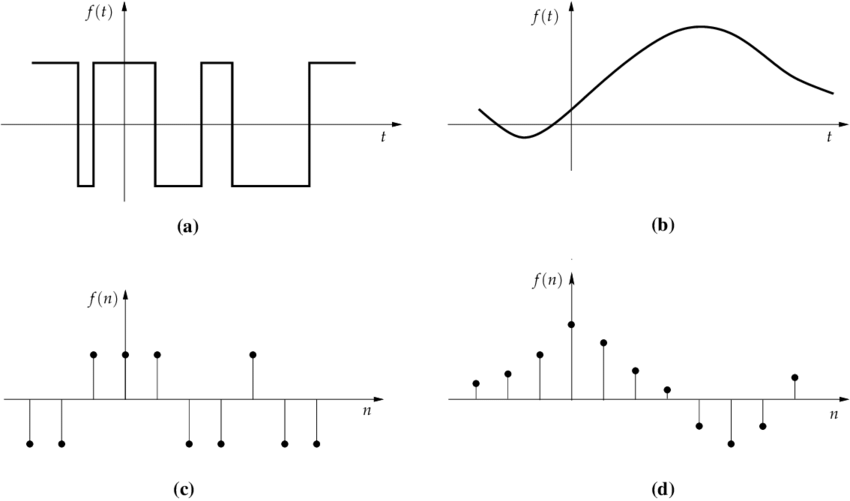
\includegraphics[scale = 0.5]{Figura-14-a-Segnale-a-valori-finiti-e-tempo-continuo-b-Segnale-continuo-a-tempo.png}
\end{figure}  

\newpage 

\section{Introduzione ai segnali} 

Per segnale si intende una funzione del tempo che rappresenta 
l'evoluzione temporale di una grandezza fisica. \newline 

Nel corso, per semplicità, saranno trattati come adimensionali, quindi senza grandezza fisica. \newline 

A partire dal segnale adimensionale, è possibile moltiplicarlo per una grandezza fisica, come ad esempio Volt o Ampere 
rispettivamente per un segnale in tensione e per un segnale in corrente. \newline 

I segnali, dal punto di vista macro, si dividono in due tipi: 

\begin{itemize}
    \item Segnali determinati 
    \item Segnali aleatori 
\end{itemize}


I segnali, sia aleatori che determinati, 
sono funzioni che possono essere a valori reali e/o a valori complessi. \newline 

Le funzioni sono continue e limitate. \newline 

I segnali determinati sono quei segnali in cui si conosce a priori il loro andamento temporale, 
quindi possiamo esplicitare il loro andamento per ogni t che va da $t = \infty$ a $t = -\infty$: 
questi segnali sono studiati grazie alla Teoria dei segnali. \newline 

Invece, i segnali aleatori sono quei segnali in cui non si conosce esplicitamente il loro andamento temporale, 
bensì, si utilizzano i concetti della Teoria della probabilità, per capire a priori la probabilità che un segnale possa essere in certi intervalli. \newline

Un segnale determinato non porta informazione perchè non ha alcuna incertezza a priori: \newline
esso è semplicemnte noto per qualunque instante di tempo. \newline 

Per essere informativo, il segnale non deve essere noto a priori. \newline 

L'obbiettivo dei sistemi di telecomunicazioni è quello di inviare informazioni, quindi soprattutto i segnali aleatori. \newline 

I segnali possono essere classificati in base alla loro variabile indipendente (generalmente il tempo) 
e alla loro grandezza che rappresentano (quindi l'ampiezza): 

\begin{itemize}
    \item Seganli a tempo continuo ed ampiezza continua 
    \item Segnali a tempo continuo ed ampiezza discreta 
    \item Segnali a tempo discreto ed ampiezza continua 
    \item Segnali a tempo discreto ed ampiezza discreta  
\end{itemize} 


\begin{figure}[h]
    \centering
    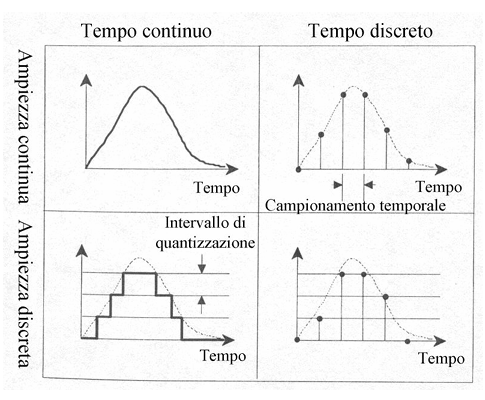
\includegraphics[scale = 0.8]{Classificazione segnali.PNG}
\end{figure}  

I segnali a tempo continuo ed ampiezza continua sono detti analogici e sono associati a fenomeni naturali (come un'onda acustica). \newline 

I segnali in cui le ampiezze sono discrete sono segnali in cui si è svolta l'operazione di quantizzazione, 
in cui il segnale reale analogico è stato trasformato in un numero. \newline 

Se anche il tempo è discreto, si definisce il segnale come digitale, che è comunemente impiegato nei sistemi digitali come i computer, microprocessori, ecc... \newline

Il processo di discretizzazione del tempo è detto campionamento. \newline 

\newpage

\section{Segnali periodici: cosa sono e quali sono i parametri utili}

I segnali periodici sono segnali che si ripetono in ogni intervallo T. \newline 

T prende il nome di periodo del seganle. \newline 

In formule matematiche, un segnale è periodico se $\forall t \in [-\infty, +\infty]$: 

{
    \Large 
    \begin{equation}
        s(t + T) = s(t)
    \end{equation}
}

Un esempio di segnale periodico: 

\begin{figure}[h]
    \centering
    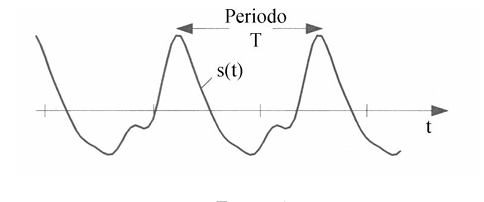
\includegraphics[scale = 0.8]{Esempio di segnale periodico.PNG}
\end{figure}  


Inoltre, viene definito come frequenza fondamentale $f_0$ l'inverso di T, cioè: 

{
    \Large 
    \begin{equation}
        f_0 = \frac{1}{T}
    \end{equation}
}

Generalmente t viene misurato in secondi, mentre la frequenza in Hertz: 

{
    \Large
    \begin{equation}
        [Hz] = \frac{1}{s}
    \end{equation}
}

In questo corso si predilisce utilizzare la pulsazione. \newline 

Si definisce la pulsazione fondamentale come: 

{
    \Large 
    \begin{equation}
        \omega_0 = 2\pi f_0
    \end{equation}
} 

e si misura in radianti al secondo: 

{
    \Large 
    \begin{equation}
        [\omega_0] = \frac{rad}{s}
    \end{equation}
}

Se il segnale è a tempo discreto, si predilisce utilizzare le parantesi quadre. \newline 

Se il segnale a tempo discreto è periodico, lo si può scrivere come: 

{
    \Large 
    \begin{equation}
        s[n + N] = s[n]
    \end{equation}
}

dove N è un numero intero. \newline 


Dato un segnale s(t) è possibile definire il suo valore medio temporale come: 

{
    \Large 
    \begin{equation}
        \overline{s(t)} 
        = 
        \lim_{\Delta T \rightarrow \infty} 
        \frac{1}{\Delta T}
        \int_{- \frac{\Delta T}{2} }^{\frac{\Delta T}{2} } 
        s(t) dt
    \end{equation}
}

In un segnale periodico: 

{
    \Large
    \begin{equation}
        \Delta T = kT
    \end{equation}
} 

Svolgendo alcuni passaggi algebrici che trovate nelle dispense del prof, avremo che: 


{
    \Large 
    \begin{equation}
        \overline{s (t)}
        = 
        \frac{1}{T} \int_{-\frac{T}{2}}^{\frac{T}{2}} 
        s(t) dt
    \end{equation}
}

Questa equazione è anche ovvia per definizione perchè, essendo un segnale periodico, se si conosce 
il suo valore medio temporale nel periodo T, lo si conosce $\forall T \in [-\infty, +\infty]$

\newpage 

\section{Delta di Dirac} 

La delta di Dirac è un impulso matematico definita come: 

{
    \Large 
    \begin{equation}
        \delta (t) 
        = 
        \lim_{\Delta t \rightarrow 0} 
        \frac{1}{\Delta t} rect_{\Delta t} (t)
    \end{equation}
}

\begin{figure}[h]
    \centering
    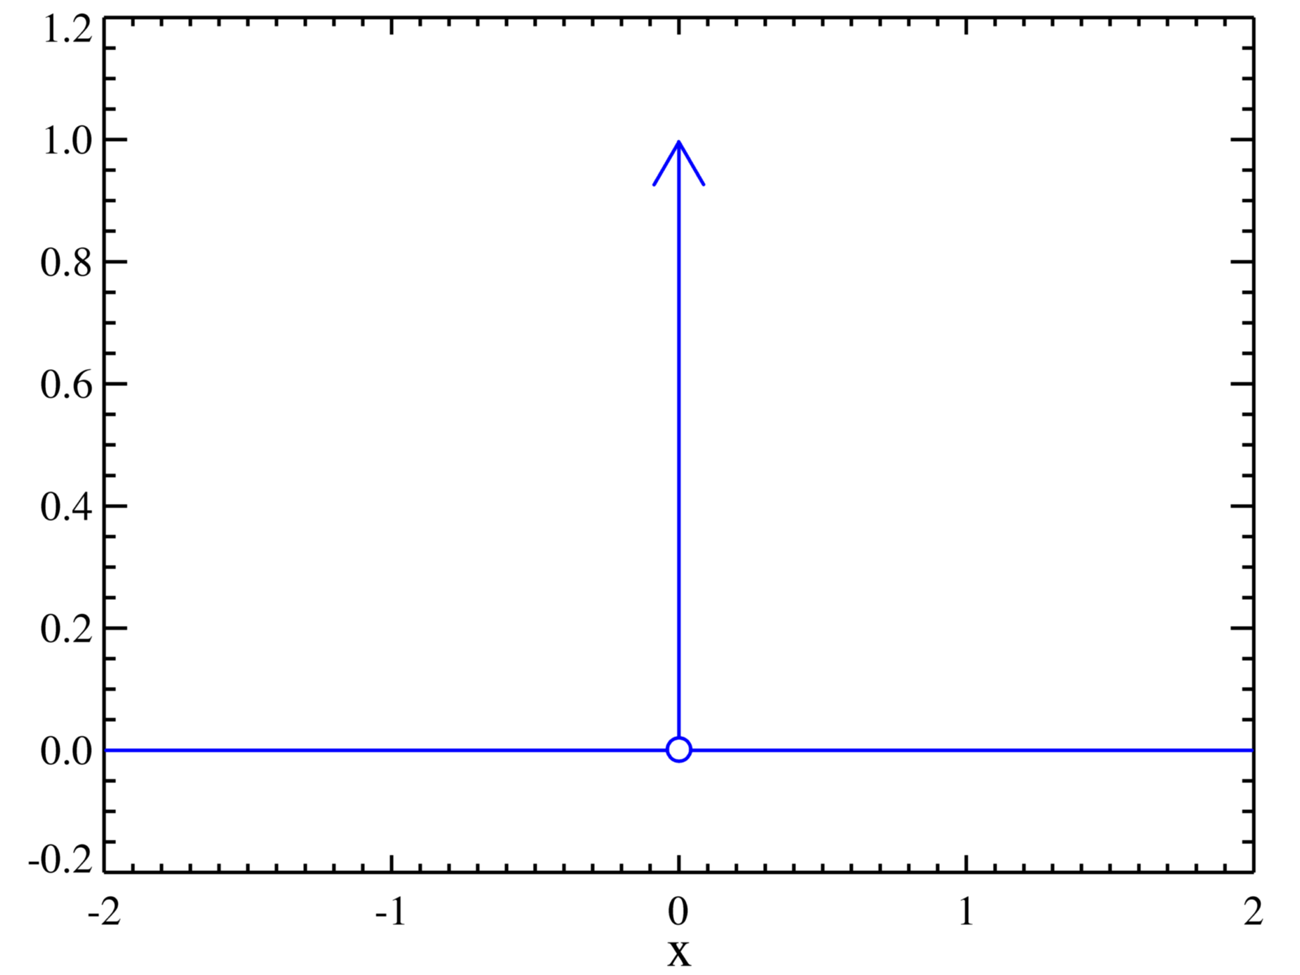
\includegraphics[scale = 0.2]{Dirac_distribution_PDF.png}
\end{figure}  

\footnote{Wikipedia - Delta di Dirac}

La Delta di Dirac gode di queste proprietà: 

{
    \Large 
    \begin{equation}
        \begin{cases}
            \delta (t = 0) = \infty \\ \\
            \delta (t \not = 0) = 0 \\ \\
            \int_{- \infty}^{ \infty} \delta (t) dt = 1
        \end{cases}
    \end{equation}
}

$\int_{- \infty}^{ \infty} \delta (t) dt = 1$ indica che l'area della Delta di Dirac è unitaria. \newline 

Se l'area è diversa da uno, basta moltiplicare la Delta di Dirac per un coefficiente moltiplicativo A. \newline 

La Delta di Dirac può trovarsi anche in un istante diverso da zero: 

{
    \Large 
    \begin{equation}
        t_0 \not = 0 
        \rightarrow 
        \delta (t - t_0)
     \end{equation}
}

o, in altri termini, possiamo vederla come una delta di Dirac shiftata nel tempo $t_0$. \newline 

Grazie alla Delta di Dirac shiftata nel tempo $t_0$, possiamo svolgere un campionamento ideale di un segnale s(t) all'instante $t_0$ come: 

{
    \Large 
    \begin{equation}
        \int_{- \infty}^{\infty} 
        s(t) \delta (t - t_0) dt 
        = 
        s(t_0)
    \end{equation}
}
\chapter{Segnali periodici nel dominio della frequenza}

\begin{figure}[h]
    \centering
    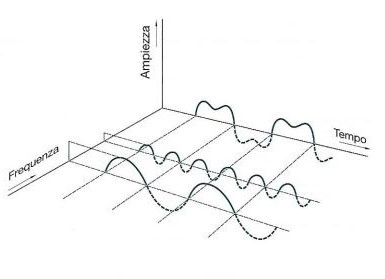
\includegraphics{Tempo frequenza segnale periodico tagliato.jpg}
\end{figure}  

\newpage 

\section{Sviluppo in serie di Fourier}

Diverse volte è utile osservare lo stesso segnale in altre rappresentazioni equivalenti. \newline 

Per rappresentazione di un segnale si intende una qualsiasi modalità idonea alla sua individuazine 
biunivoca. \newline 

La rappresentazione può comportare un cambiamento del dominio di definizione. \newline  

Quindi, grazie ad una rappresentazione, si può passare da un dominio all'altro dello stesso segnale. \newline 

Se il segnale s(t) è periodico con periodo T e pulsazione fondamentale $\omega_0$, possiamo definire una rappresentazione 
nota come Sviluppo in serie di Fourier. \newline 

Il dominio non sarà il tempo, bensì la frequenza (cioè l'inverso del tempo). \newline 

s(t) può essere visto come, grazie alla formula di sintesi dello sviluppo in serie di Fourier: \newline

{
    \Large 
    \begin{equation}
        s(t) 
        = 
        \sum_{k = - \infty}^{\infty} 
        C_k \frac{1}{\sqrt{T}} e^{\jmath \kappa \omega_0 t}
    \end{equation}
}

in cui: \newline

{
    \Large 
    \begin{equation}
        \omega_0 = \frac{2 \pi}{T}
    \end{equation}
}

e $C_k$ viene calcolato dall'analisi dello sviluppo in serie di Fourier: \newline

{
    \Large 
    \begin{equation}
        C_k 
        =
        \frac{1}{\sqrt{T}} \int_{-\frac{T}{2}}^{\frac{T}{2}} 
        s(t) e^{- \jmath \kappa \omega_0 t} dt
    \end{equation}
}

Ricordando, dalla matematica: 

{
    \Large 
    \begin{equation}
        \jmath ^{2} = -1 
    \end{equation}
}


 $e^{\jmath \kappa \omega_0 t}$ rappresenta una sinusoide e ponendo: 

{
    \Large 
    \begin{equation}
        \omega_k = k \omega_0
    \end{equation}
}

possiamo dire che qualsiasi segnale s(t) può essere visto come una 
successione di sinusoidi di diversa pulsazione. \newline 

In formule: 

{
    \Large 
    \begin{equation}
        s(t) \leftrightarrow \{C_k\}
    \end{equation}
}

dove per $\{C_k\}$ si intendene la lista dei coefficienti che formulano il segnale s(t). \newline 


Siccome $\{C_k\}$ sono dei coefficienti che rappresentano delle sinusoidi, 
i coefficienti avranno una parte reale e una parte immmaginaria. \newline 

Il singolo coefficiente $C_k$ avrà la parte reale, 
scritta come $\Re[C_k]$ oppure $\abs{C_k}$, e la parte immmaginaria del coeffieciente 
sarà indicata come $\Im[C_k]$ oppure $\arg[C_k]$. \newline 

$\abs{C_k}$ prende anche il nome di modulo di $C_k$, 
mentre $\arg[C_k]$ prende il nome di fase di $C_K$. \newline 

Dal punto di vista grafico, possiamo visualizzare tutti i moduli e le fasi dei coeffiecienti $C_k$ 
usando lo spettro. \newline 

Lo spettro dei moduli di $C_k$ prende il nome di spettro di ampiezza, 
mentre lo spettro delle fasi prende il nome di spettro di fase. \newline 

Un esempio di spettro di ampiezza e spettro di fase: 

\begin{figure}[h]
    \centering
    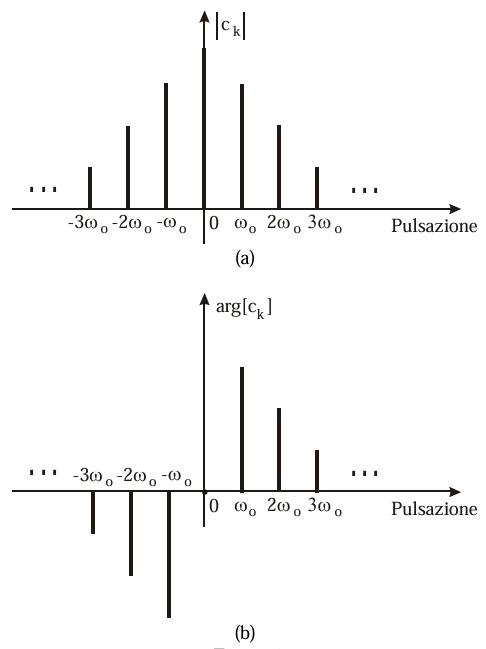
\includegraphics{Esempio di spettro di ampiezza e di fase.PNG}
\end{figure} 

Come si vede dalla figura, nello sviluppo in serie di Fourier, 
gli spettri sono a righe perchè le armoniche sono discrete, armoniche multiple della frequenza fondamentale. \newline 

Con i puntini si intendono armoniche infinite, nella realtà si prenderanno le armoniche significative.  

\newpage 

\section{Criterio di Dirichlet} 

Dal punto di vista matematico, non tutti i segnali periodici possono essere rappresentati 
usando la rappresentazione della serie di Fourier. \newline 

Il segnale s(t) deve soddisfare il criterio di Dirichlet cioè: 

\begin{itemize}
    \item se s(t) è assolutamente integrabile sul periodo T, o in formula: 
    \begin{equation}
        \int_{-\frac{T}{2}}^{\frac{T}{2}} \abs{s(t)} dt < \infty
    \end{equation}
    \item se s(t) è continua o presenta un numero finito di punti di discontinuità di prima specie 
    \item se s(t) presenta in un periodo T un numero finito di massimi e minimi 
\end{itemize}

allora, se s(t) soddisfa questi criteri, la serie di Fourier converge al valore assunto dalla funzione
s(t) nei punti in cui questa è continua e alla semisomma del limite destro e sinitro nei punti in cui s(t) presenta le 
eventuali discontinuità di prima specie. \newline 

I segnali che vedremo nel corso soddisferanno il criterio di Dirichlet. \newline  

\newpage    

\section{Ortogonalità tra due segnali} 

Due segnali $x_1 (t)$ e $x_2 (t)$, in genere complessi, risultano ortogonali 
nell'intervallo $A \le t \le B$ se: 

{
    \Large 
    \begin{equation}
        \int_{A}^{B} 
        x_1 (t) x_2 ^{*} (t) dt = 0 
    \end{equation}
}

in cui il simbolo $*$ indica l'operazione di coniugato complesso. \newline 

Un esempio di sequenze ortogonali: 

\begin{figure}[h]
    \centering
    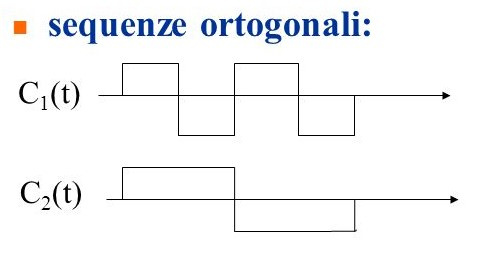
\includegraphics[scale = 0.8]{Segnali ortogonali.jpg}
\end{figure}  

Possiamo avere anche che: 

{
    \Large 
    \begin{equation}
        \begin{cases}
            A = -\infty \\
            B = \infty
        \end{cases} 
    \end{equation}
} 

Nel caso specifico, la condizione di ortogonalità tra due generiche funzioni espansione 
è verificata: 

{
    \Large 
    \begin{equation}
        \int_{-\frac{T}{2}}^{\frac{T}{2}} 
        e^{\jmath \kappa \omega_0 t} e^{-\jmath h \omega_0 t} 
        = 
        \begin{cases}
            T \text{    se  } h = k\\ 
            0 \text{    se  } h \neq k 
        \end{cases}
    \end{equation}
}

Questa equazione è valida solo se s(t) è un segnale reale. \newline 

\newpage

\section{Come ricavare moduli e fase in una serie di Fourier} 

Grazie alle formule di Eulero, possiamo scrivere la formula di sintesi della Serie di Fourier da: 

{
    \Large 
    \begin{equation}
        s(t) 
        = 
        \sum_{\kappa = - \infty}^{\infty} 
        C_k \frac{1}{\sqrt{T}} e^{\jmath \kappa \omega_0 t}
    \end{equation}
} 

Essendo un segnale s(t) reale, e che quindi per $\kappa \le 0$ si rispecchia quello che succede in $\kappa \ge 0$, 
la sommatoria possiamo scriverla da $\kappa \ge 0$, cioè: 

{
    \Large 
    \begin{equation}
        s(t) = \frac{a_0}{2} 
        +
        \sum_{\kappa = 1}^{+ \infty} [a_\kappa \cos(\kappa \omega_0 t) + b_\kappa \sin(\kappa \omega_0 t)] 
    \end{equation}
} 

o in alternativa: 

{
    \Large 
    \begin{equation}
        s(t) 
        = 
        \frac{A_0}{2} 
        + 
        \sum_{\kappa = 1}^{+ \infty} A_\kappa \cos(\kappa \omega_0 t - \phi_\kappa)   
    \end{equation}
}

Per ricavare i coeffiecienti indicati nelle equazioni, possiamo usare le prossime equazioni: 

{
    \Large 
    \begin{equation}
        a_0  
        = 
        \frac{2}{\sqrt{T}} C_0 
        = 
        \frac{2}{T} \int_{-\frac{T}{2}}^{\frac{T}{2}} s(t) dt 
    \end{equation}
} 


{
    \Large 
    \begin{equation}
        a_\kappa  
        = 
        \frac{2}{\sqrt{T}} \Re[C_\kappa]
        = 
        \frac{2}{T} \int_{-\frac{T}{2}}^{\frac{T}{2}} s(t) \cos(\kappa \omega_0 t) dt 
    \end{equation}
} 

{
    \Large 
    \begin{equation}
        b_\kappa  
        = 
        -\frac{2}{\sqrt{T}} \Im[C_\kappa]
        = 
        \frac{2}{T} \int_{-\frac{T}{2}}^{\frac{T}{2}} s(t) \sin(\kappa \omega_0 t) dt 
    \end{equation}
} 

{
    \Large 
    \begin{equation}
        A_\kappa  
        = 
        \sqrt{a_\kappa ^{2} + b_\kappa ^{2}} 
    \end{equation}
} 

{
    \Large 
    \begin{equation}
        \arctan(\frac{b_\kappa}{a_\kappa})
    \end{equation}
}

Se il segnale è reale, è molto utile perchè gode di simmetria: 
\begin{itemize}
    \item se s(t) è reale pari, quindi per un qualsiasi t, 
    {
        \Large 
        \begin{equation}
            s(-t) = s(t)
        \end{equation}
    
    }
    
    lo sviluppo in serie di Fourier sarà anche pari, quindi si svolgeranno gli $a_k$ in cui è presente un $\cos(\kappa \omega_0 t)$
    
    \item  se s(t) è reale dispari, quindi per un qualsiasi t, 
    {
        \Large 
        \begin{equation}
            s(-t) = -s(t)
        \end{equation}
    } 
    lo sviluppo in serie di Fourier sarà anche dispari, quindi si svolgeranno gli $b_k$ in cui è presente un $\sin(\kappa \omega_0 t)$ \newline
\end{itemize}

Se s(t) ha valore medio nullo, allora: 

{
    \Large 
    \begin{equation}
        C_0 = a_0 = A_0 = 0
    \end{equation}
} 

\newpage 

\section{Proprietà dello sviluppo di una serie di Fourier} 


Se s(t) è un segnale periodico e soddisfa il criterio di Dirichlet, allora possiamo 
rappresentarlo nello sviluppo di una serie di Fourier. \newline 

Considerando un segnale s(t) rappresentato in uno sviluppo di una serie di Fourier, il nuovo segnale $s^{'} (t)$ gode delle seguenti proprietà: \newline 

\textbf{Proprietà della traslazione temporale} 

Considerando $\tau$ un tempo costante, allora: 

{
    \Large 
    \begin{equation}
        s^{'} (t) = s(t - \tau)
        \leftrightarrow
        c_\kappa ^{'}  = c_\kappa e^{-\jmath \kappa \omega_0 \tau} 
    \end{equation}
    \newline
}

 

\textbf{Proprietà della traslazione in frequenza} 

Considerando: 

{
    \Large
    \begin{equation}
        \omega_A = n \omega_0
    \end{equation}
} 

in cui n è un numero, allora: 

{
    \Large 
    \begin{equation}
        s^{'} (t) = s(t) e^{\jmath \omega_A t} 
        \leftrightarrow 
        c_\kappa ^{'} = c_{\kappa - n}
    \end{equation}
}

\textbf{Proprietà di inversione dell'asse temporale} 

{
    \Large 
    \begin{equation}
        s^{'} (t) = s(-t) 
        \leftrightarrow
        c_\kappa ^{'} = c_{-\kappa}
    \end{equation}
} 

\textbf{Proprietà del coniugo} 

{
    \Large 
    \begin{equation}
        s^{'} (t) = s^{*} (-t) 
        \leftrightarrow
        c_\kappa ^{'} = c_{-\kappa} ^{*}
    \end{equation}
} 

\textbf{Proprietà della derivazione} 

Considerando m un coefficiente di un numero intero, 

{
    \Large
    \begin{equation}
        s^{'} (t) = \frac{d ^{m} s(t)}{dt^{m}}
        \leftrightarrow 
        c_\kappa ^{'} = c_{-\kappa} (\jmath \kappa \omega_0)^{m}
    \end{equation}
}

\textbf{Proprietà dell'integrazione}

Se il valore medio del segnalo è nullo, cioè: 

{
    \Large 
    \begin{equation}
        c_0 
        = \frac{1}{\sqrt{T}} 
        \int_{-\frac{T}{2}}^{\frac{T}{2}}
        s(t) dt 
        = 
        0
    \end{equation}
}

allora: 

{
    \Large
    \begin{equation}
        s^{'} (t) = \int_{-\frac{T}{2}}^{t} s(t) dt 
        \leftrightarrow 
        \begin{cases}
            c_0 ^{'} = \sum_{\kappa \neq 0 } \frac{c_\kappa}{\jmath \kappa \omega_0} (-1)^{\kappa} \\ \\
            c_\kappa ^{'} = \frac{c_\kappa}{\jmath\kappa \omega_0}
        \end{cases}
   \end{equation}
}

\textbf{Proprietà di linearità}

Considerando due segnali $s_1 (t)$ e $s_2 (t)$, di periodo T con i rispettivi coefficienti dello sviluppo 
della serie di Fourier $c_{1\kappa}$ e $c_{2\kappa}$: 

{
    \Large
    \begin{equation}
        s(t) ^{'} = A_1 s_1 (t) + A_2 s_2 (t)
        \leftrightarrow 
        c_\kappa ^{'} = A_1 c_{1\kappa} + A_2 c_{2\kappa}  
    \end{equation}
}

\textbf{Proprietà della convoluzione} 

Considerando la convoluzione tra i due segnali nel periodo T, 

{
    \Large 
    \begin{equation}
        C(t) = \int_{-\frac{T}{2}}^{\frac{T}{2}} s_1 (\tau) s_2 (t - \tau) d\tau 
        \leftrightarrow 
        c_\kappa ^{'} = c_{1\kappa} c_{2\kappa} \sqrt{T}
    \end{equation}
} 


\begin{tcolorbox}
    Per visualizzare graficamente cosa significa fare una convoluzione, ti lascio un video: \newline 
    But what is a convolution? by 3Blue1Brown \newline
    \url{https://www.youtube.com/watch?v=KuXjwB4LzSA&t=129s}    
\end{tcolorbox}

\textbf{Proprietà del prodotto}

{
    \Large
    \begin{equation}
        s^{'} (t) = s_1 (t) s_2(t) 
        \leftrightarrow 
        c_\kappa ^{'} = \frac{1}{\sqrt{T}} \sum_{h = - \infty}^{+ \infty} c_{1 h} c_{2(\kappa - h)}
    \end{equation}
}

Questa proprietà può essere vista anche come convoluzione discreta tra ${c_{1\kappa}}$ e ${c_{2\kappa}}$ \newline 

\newpage
.
\newpage
.
\newpage

 
\chapter{Segnali aperiodici nel dominio della frequenza}

\begin{figure}[h]
    \centering
    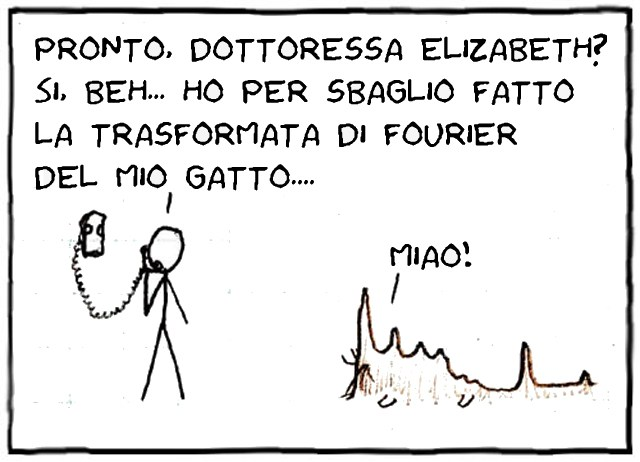
\includegraphics[scale = 3]{meme a caso.jpg}
\end{figure}  

\newpage 

\section{Trasformata di Fourier}

Dai segnali periodici del capitolo precedente, passiamo ora ai segnali aperiodici. \newline 

I segnali aperiodici possono essere visti come segnali periodici con T che tende ad infinito:  

{
    \Large 
    \begin{equation}
        T \rightarrow + \infty 
        \leftrightarrow 
        \omega_0 \rightarrow 0
    \end{equation}
}

Non possiamo definire uno sviluppo in serie di Fourier, bensì la nuova rappresentazione 
per un segnale aperiodico si chiamerà trasformata di Fourier definita come: 

{
    \Large 
    \begin{equation}
        S(\omega) = F[s(t)] = \int_{-\infty}^{+\infty} s(t) e^{-\jmath \omega t} dt 
    \end{equation}
}

L'anti-trasformata di Fourier, cioè l'inverso della trasformata di Fourier, è definito come: 

{
    \Large 
    \begin{equation}
        s(t) = F^{-1} [S(\omega)] = \frac{1}{2 \pi} \int_{-\infty}^{+\infty} S(\omega) e^{\jmath \omega t} d\omega
    \end{equation}
}

Quindi possiamo vedere lo stesso segnale come: 

{
    \Large
    \begin{equation}
        s(t) 
        \leftrightarrow 
        S(\omega)
    \end{equation}
}

Come lo sviluppo in serie di Fourier, possiamo definire lo spettro di ampiezza e di fase 
per una trasformata di Fourier: 

{
    \Large 
    \begin{equation}
        S(\omega) = \abs{S(\omega)} e^{\jmath \theta_s (\omega)}
    \end{equation}
}

A differenza della serie di Fourier, gli spettri non saranno a righe, bensì continui. \newline 

\newpage 

\section{Caratteristiche di un segnale Fourier trasformabile} 

Come nel caso dei segnali in serie di Fourier, 
non tutti i segnali possono essere Fourier trasformabili. \newline 

I segnali devono essere assolutamente integrabili: 

{
    \Large 
    \begin{equation}
        \int_{-\infty}^{+\infty} \abs{s(t)} dt < \infty
    \end{equation}
} 

I segnali che sono assolutamente integrabili vengono detti impulsivi. \newline 

Se il segnale s(t) è reale: 

{
    \Large
    \begin{equation}
        \begin{cases}
            \Re[S(-\omega)] = \Re[S(\omega)] \\ 
            \Im [S(-\omega)] = -\Im[S(\omega)]
        \end{cases}
        \leftrightarrow
        \begin{cases}
            \abs{S(-\omega)} = \abs{S(\omega)} \\ 
            \theta_s (-\omega) = - \theta_s (\omega)
        \end{cases}
    \end{equation}
}

dove: 
{
    \Large 
    \begin{equation}
        \Re[S(\omega)] = \int_{-\infty}^{+\infty} s(t) \cos(\omega t ) dt
    \end{equation}
}

{
    \Large 
    \begin{equation}
        \Im[S(\omega)] = \int_{-\infty}^{+\infty} - s(t) \sin(\omega t ) dt
    \end{equation}
}

Se s(t) è reale pari, la sua trasformata è reale pari:

{
    \Large 
    \begin{equation}
        \Re[S(\omega)] = \Re[S(-\omega)]
    \end{equation}
}

{
    \Large 
    \begin{equation}
        \Im[S(\omega)] = 0
    \end{equation}
}

Se s(t) è reale dispari, la sua trasformata è immaginaria dipari:

{
    \Large 
    \begin{equation}
        \Re[S(\omega)] = 0
    \end{equation}
}

{
    \Large 
    \begin{equation}
        \Im[S(\omega)] = -\Im[S(-\omega)] 
    \end{equation}
}


\newpage 

\section{Proprietà della trasformata di Fourier} 

Anche questo tipo di rappresentazione, ammette delle proprietà: \newline 

\textbf{Proprietà della traslazione temporale} 

{
    \Large
    \begin{equation}
        s^{'} (t) = s(t - \tau) 
        \leftrightarrow 
        S^{'} (\omega) = S(\omega) e^{-\jmath \omega \tau}
    \end{equation}
}

\textbf{Proprietà della traslazione in frequenza}

Considerando $\omega_1$ la frequenza traslata, possiamo dire che: 

{
    \Large 
    \begin{equation}
        s^{'} (t) = s(t) e^{\jmath \omega_1 t} 
        \leftrightarrow 
        S^{'} (\omega) = S(\omega -\omega_1)
    \end{equation}
}


\textbf{Proprietà di inversione dell'asse temporale}

{
    \Large 
    \begin{equation}
        s^{'} (t) = s (-t)
        \leftrightarrow 
        S^{'} (\omega) = S(\omega)
    \end{equation}
}

\textbf{Proprietà del coniugo}

{
    \Large
    \begin{equation}
        s^{'} (t) = s^{*} (t)
        \leftrightarrow 
        S^{'} = S^{*} (-\omega)
    \end{equation}
}

\textbf{Proprietà della derivazione}

{
    \Large
    \begin{equation}
        s^{'} (t) = \frac{d^{m} s(t)}{dt^{m}}
        \leftrightarrow
        S^{'} (\omega) = S(\omega) (\jmath \omega) ^{m}
    \end{equation}
}

\textbf{Proprietà dell'integrazione} 

Se il valore medio è nullo:

{
    \Large 
    \begin{equation} 
        S(\omega = 0) = \int_{- \infty}^{+ \infty} s(t) dt = 0
    \end{equation}
}

allora: 

{
    \Large 
    \begin{equation}
        S^{'} (t) = \int_{- \infty}^{t} s(t) dt 
        \leftrightarrow
        S^{'} (\omega) = \frac{S(\omega)}{\jmath \omega}
    \end{equation}
}

Grazie alla proprietà dei segnali impulsivi, quindi all'introduzione della Delta di Dirac, 
possiamo definire la trasformata di Fourier generalizzata anche per segnali con valore medio non nullo: 

{
    \Large 
    \begin{equation}
        s^{'} (t) = \int_{- \infty}^{t} s(t) dt 
        \leftrightarrow 
        S^{'} (\omega) = \frac{S(\omega)}{\jmath \omega} + \pi S(\omega = 0) \delta(\omega)
    \end{equation}
}

\textbf{Proprietà della moltiplicazione per t}

{
    \Large
    \begin{equation}
        s^{'} (t) = t ^{m} s(t) 
        \leftrightarrow
        S^{\omega} = \jmath ^{m} \frac{d^{m} S(\omega)}{d\omega ^{m}}
    \end{equation}
}

\textbf{Proprietà di dualità}

Dato un segnale s(t) la cui trasformata sia $S(\omega)$, la trasformazione di S(t) risulta 
$2\pi s(-\omega)$: 

{
    \Large 
    \begin{equation}
        s(t) \leftrightarrow S(\omega) 
        \text{  implica } 
        S(t) \leftrightarrow 2\pi s(-\omega)
    \end{equation}
}

Questa proprietà è molto importante perchè l'andamento del segnale di inizio del tempo alla 
rappresentazione in trasformata di Fourier è uguale all'andamento del segnale da trasformata 
di Fourier al segnale nel tempo sono uguali a meno di un fattore di $2 \pi$. \newline 

Quindi t e $\omega$ sono interscambiali. \newline 


\textbf{Proprietà di linearità} 

{
    \Large 
    \begin{equation}
        s^{'} (t) = A_1 s_1(t) + A_2 s_2(t) 
        \leftrightarrow 
        S^{'} (\omega) = A_1 s_1(\omega) + A_2 s_2(\omega)
    \end{equation}
} 

\textbf{Proprietà della convoluzione} 

{
    \Large 
    \begin{equation}
        \begin{split}
            c(t) 
            &= \int_{- \infty}^{+\infty} s_1(\tau) s_2(t-\tau) d\tau 
            \\
            &= s_1 (t) \otimes s_2 (t) \\
            &\updownarrow 
            \\ 
           C(\omega) &= S_1(\omega) S_2(\omega)    
        \end{split}
    \end{equation}
}

L'integrazione viene svolta su $\tau$ e t viene visto come parametro nella formula di integrazione. \newline 

\textbf{Proprietà del prodotto}

{
    \Large 
    \begin{equation}
        s^{'} (t) = s_1(t) s_2 (t) 
        \leftrightarrow 
        S^{'}(\omega) = \frac{1}{2 \pi} \int_{-\infty}^{\infty}S_1(\theta) S_2 (\omega - \theta) d\theta
    \end{equation}
}

L'integrazione viene svolta su $\theta$ e $\omega$ viene visto come parametro nella formula di integrazione. \newline 

A meno della costante $\frac{1}{2 \pi}$, questa proprietà si dimostra grazie alla proprietà di dualità. \newline 

\newpage 

\section{Altre caratteristiche sulla dualità tempo-frequenza} 

Di seguito verranno elencate alcune caratteristiche sulla dualità tempo-frequenza. \newline 

{
    \begin{itemize}
        \item Un segnale s(t) che è limitato nel tempo, ha spettro illimitato sull'asse delle pulsazioni 
        \item Un segnale con spettro delle pulsazioni limitato, ha un'evoluzione temporale illimitata in t. \\ 
        (Questo si dimostra grazie alla proprietà di dualità tempo-frequenza spiegato nella sezione precedente) 
        \item Possiamo definire $B_\omega$ la larghezza significativa di un segnale, cioè l'intervallo di pulsazioni in cui il modulo di $S(\omega)$ assume valori non trascurabili, maggiori di una soglia minima prefissata: \\ 
        quanto maggiore risulta $B_\omega$, s(t) varierà più rapidamente. 
        \item Possiamo definire $D_t$ la durata significativa come l'intervallo di tempo in cui il segnale assume valori non trascurabili e definiamo Q come parametro di qualità. \\
        In formule: 
        {
            \Large 
            \begin{equation}
                B_\omega D_t \geq Q
            \end{equation}
        } 
        Generalmente: 
        {
            \Large 
            \begin{equation}
                Q = 2\pi
            \end{equation}
        } 
        
    \end{itemize}
}


\newpage 

\section{Teorema del cambiamento di scala} 

Un teorema che è importante sulla dualità tempo-frequenza è il seguente. \newline 


Consideriamo il segnale: 

{
    \Large 
    \begin{equation}
        y(t) = s(\alpha t)
    \end{equation}
}

Se consideriamo $S(\omega)$ la trasformata di Fourier di s(t), e $\alpha$ un parametro. \newline 

Al cambiare di $\alpha$, ci saranno degli effetti diversi sullo spettro di $S(\omega)$ : 

\begin{itemize}
    \item $\abs{\alpha} > 1 \rightarrow $ compressione della scala dei tempi 
    \item  $\abs{\alpha} < 1 \rightarrow $ dilatazione della scala dei tempi 
    \item $\alpha < 0 \rightarrow $ inversione della scala dei tempi 
\end{itemize}

Facendo la trasformata di Fourier di y(t), avremo che: 
{
    \Large 
    \begin{equation}
        y(t) = s(\alpha t) 
        \leftrightarrow 
        Y(\omega) = \frac{1}{\abs{\alpha}} S(\frac{\omega}{\alpha})
    \end{equation}
} 

Si nota che una dilatazione dell'asse dei tempi comporta una compressione dell'asse delle pulsazioni e viceversa. \newline 

\newpage 

\section{Teorema della modulazione} 

Consideriamo il segnale originale s(t) e consideriamo il nuovo segnale $s^{'} (t)$ e la sua trasformata di Fourier come: 

{
    \Large 
    \begin{equation}
        \begin{split}
            s^{'} (t) &= s(t)\cos(\omega_0 t) \\ 
            &\updownarrow \\
            S^{'} (\omega) &= \frac{1}{2} [S(\omega - \omega_0) + S(\omega + \omega_0)]    
        \end{split}
    \end{equation}
}

\subsection{Dimostrazione del teorema della modulazione} 

Utilizzando la formula di Eulero e l'argomento $\omega_0 t$: 

{
    \Large 
    \begin{equation}
        e^{\jmath \omega_0 t} = \cos(\omega_0 t) + \jmath \sin(\omega_0 t) = \jmath(-1)^{\omega_0 t}
    \end{equation}
}

Possiamo riscrivere: 

{
    \Large 
    \begin{equation}
        s^{'} (t) = s(t)\cos(\omega_0 t)
        \leftrightarrow 
        s^{'} (t) = s(t) \frac{e^{\jmath \omega_0 t} + e^{-\jmath \omega_0 t}}{2}
    \end{equation}
} 

Di qui, applicando le proprietà di linearità e di traslazione in frequenza, si ottiene: 

{
    \Large 
    \begin{equation}
        \begin{split}
            S^{'} (\omega) 
        &= 
        \frac{S (\omega - \omega_0) + S (\omega + \omega_0)}{2}
        \\ 
        &= 
        \frac{1}{2}
        [S (\omega - \omega_0) + S (\omega + \omega_0)]
        \end{split}
    \end{equation}
}

\newpage 

\subsection{Considerazioni sul teorema della modulazione} 

Dal teorema della modulazione, notiamo che se la trasformata di Fourier del segnale s(t) si espande 
nella banda $[- \omega_B, +\omega_B]$, lo stesso segnale si troverà centrato a destra in $\omega_0$ con banda 
$[\omega_0 - \omega_B, \omega_0 + \omega_B]$, lo stesso accade a sinistra dello spettro. \newline 

Il segnale sarà lo stesso di quello originario centrato in $- \omega_0$ e $\omega_0$ moltiplicato per $\frac{1}{2}$. \newline 

La figura seguente, spiega il teorema dal punto di vista grafico: 

\begin{figure}[h]
    \centering
    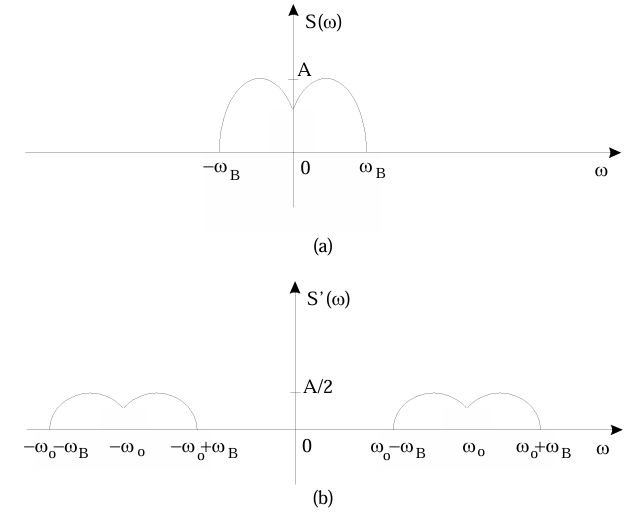
\includegraphics[scale = 1]{Teorema della modulazione visto graficamente.PNG}
\end{figure}  

La figura in alto viene definita come il segnale in banda base, cioè la banda in cui è s(t);  
mentre $S^{'} (\omega)$ viene definita come il segnale in banda traslata. \newline 

La porzione di spettro in cui $\abs{\omega} > \omega_0$  viene definita come banda laterale superiore, 
mentre la porzione di spettro per $\abs{\omega} < \omega_0$ prende la banda laterale inferiore. \newline 

Se il segnale s(t) è reale, allora le due sottobande godono di simmetria e lo spettro complessivo è simmetrico rispetto all'origine. \newline 

\newpage 

\include{4 - Proprietà di correlazione}
\chapter{Sistemi lineari} 

\begin{figure}[h]
    \centering
    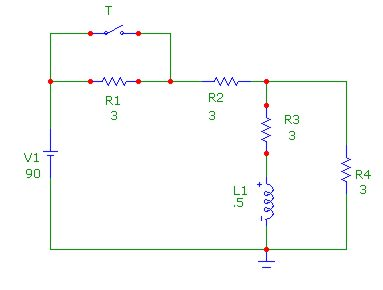
\includegraphics[scale = 1]{esempio di sistema lineare.jpeg}
\end{figure}  

\newpage 

\section{Cosa è un sistema lineare e cosa rappresenta} 

È detto sistema lineare un sistema descritto da un'equazione integro-differenziale 
lineare, che leghi un segnale di ingresso x(t) (detto anche sollecitazione) 
al corrispondente segnale in uscita (o risposta) y(t). \newline 

Se l'equazione integro-differenziale è a coefficienti costanti, 
il sistema risulta invariante nel tempo (detto anche sistema permanente). \newline 

Il problema fondamentale consiste nel determinare l'evoluzione dell'uscita y(t) a partire dalla conoscenza 
dell'ingresso x(t). \newline 

{
    \begin{figure}[h]
        \centering
        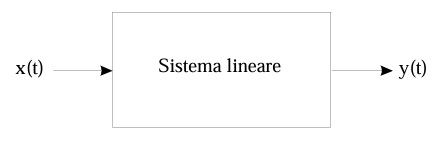
\includegraphics[scale = 1]{Blocco sistema lineare.PNG}
    \end{figure}  
     
}

Il problema consiste nel descrivere opportunatamente il blocco lineare intermedio e nel mettere in relazione 
le due funzioni x(t) e y(t). \newline 

I sistemi lineari sono molto comodi perchè, grazie al principio della sovrapposzione, 
è possibile sapere y(t) come combinazione lineare di $y_1(t)$ e $y_2(t)$, che, rispettivamente, 
sono le uscite dei segnali di ingresso $x_1(t)$ e $x_2(t)$. \newline 

Grazie alla proprietà di campionamento della delta di Dirac, possiamo scrivere che: 

{
    \Large 
    \begin{equation}
        x (t) 
        = 
        \int_{- \infty}^{+ \infty} 
        x (\tau) \delta(t - \tau) d\tau
    \end{equation}
}

Questa formula ci spiega che x(t) può essere vista come somma di un'infinità non numerabili di impulsi matematici 
$\delta (t - \tau)$ disposti in $t = \tau$ di area pari a $x(\tau) d\tau$, $\tau$ varia da $[-\infty, +\infty]$. \newline 

Indichiamo con h(t) la risposta del sistema ad un impulso matematico in $t=0$, cioè: 

{
    \Large 
    \begin{equation}
        y(t) = h(t) \leftrightarrow x(t) = \delta(t)
    \end{equation}
}

Se il sistema è permanente, la risposta ad un impulso matematico allocata in $t = \tau$ sarà $h(t - \tau)$. \newline 

Grazie al principio della sovrapposzione degli effetti, possiamo scrivere che: 

{
    \Large 
    \begin{equation}
        y(t) = \int_{-\infty}^{+\infty}
        x(\tau) h (t - \tau) d\tau
    \end{equation}
}

y(t) esprime la relazione ingresso-uscita ed è chiaramente un integrale di convoluzione. \newline 

Quindi possiamo applicare tutte le proprietà che abbiamo visto nei capitoli precedenti. \newline 

Possiamo esprimere la risposta impulsiva di un sistema come: 

{
    \Large 
    \begin{equation}
        y(t) = x(t) * h(t)
    \end{equation}
}

\begin{tcolorbox}
Nel corso degli appunti, $\otimes$  o * saranno segni interscambiali per indicare una convoluzione tra i segnali     
\end{tcolorbox}

Come visto nella convoluzione, è conveniente esprimere e fare i calcoli in frequenza piuttosto che nel tempo. \newline 

La trasformata dell'uscita y(t) sarà: 

{
    \Large 
    \begin{equation}
        Y(\omega) = X(\omega)H(\omega) 
    \end{equation}
}

in cui $Y(\omega)$,  $X(\omega)$ e $H(\omega)$ sono rispettivamente le trasformate di Forurier 
dell'uscita, dell'ingresso e della risposta impulsiva del sistema. \newline 

Sapendo $Y(\omega)$ è possibile riportare l'uscita nel dominio del tempo, anti-trasformando $Y(\omega)$: 

{
    \Large 
    \begin{equation}
        y (t)= F^{-1} [Y(\omega)] = F^{-1} [X(\omega) H(\omega) ] 
    \end{equation}
}

La funzione $H(\omega)$ prende il nome di funzione di trasferimento del sistema. \newline 

$H(\omega)$ modifica lo spettro del segnale di ingresso, eliminando parte dello spettro originale: 
ecco perchè un sistema lineare viene definito anche come filtro. \newline 

Idealmente, le frequenze che passano nel filtro non sono modificate dal sistema-lineare, 
nella realtà ci saranno alcune modifiche. \newline 


Quindi, possiamo dividere i filtri in due categorie: 

\begin{itemize}
    \item filtri fisicamente realizzabili 
    \item filtri idealmente realizzabili 
\end{itemize} 

In un filtro vero, vale a dire costruito con componenti reali, la risposta non può precedere la sollecitazione. \newline 

Sapendo che h(t) è la risposta impulsiva in $t=0$, ciò comporta che, in un filtro "vero" debba essere: 

{
    \Large 
    \begin{equation}
        h(t) = 0 \text{ per } t < 0 
    \end{equation}
} 

Questa proprietà va sotto il nome di principio di causalità e rappresenta la condizione necessaria affinche
un filtro idealmente lo sia anche fisicamente. \newline 

\newpage 


\section{Densità spettrale di energia e di potenza in un filtro} 

Essendo: 

{
    \Large 
    \begin{equation}
        Y(\omega) = H(\omega) X(\omega)
    \end{equation}
}

le densità spettrali di energia (ove applicabili) dei segnali in ingresso e in uscita sono tra 
loro legate dalla seguente relazione: 

{
    \Large 
    \begin{equation}
        \abs{Y(\omega)} ^{2} 
        = 
        \abs{H(\omega) X(\omega)} ^{2} 
        = 
        \abs{H(\omega)} ^{2} \cdot \abs{X(\omega)} ^{2}
    \end{equation}
}

Una relazione analoga vale per gli spettri di potenza, indicati con $p_x (\omega)$ 
(per l'ingresso) e $p_y (\omega)$ (per l'uscita): 

{
    \Large 
    \begin{equation}
        p_y (\omega) = \abs{H(\omega)} ^{2} p_x (\omega)
    \end{equation}
}

Dunque, la densità in uscita si ottiene moltiplicando la densità in ingresso 
per il modulo al quadrato della funzione di trasferimento. \newline 

Sapendo la relazione tra densità spettrale e funzione di auto-correlazione di un segnale, possiamo 
conoscere la relazione ingresso-uscita anche nel dominio del tempo. \newline 

Anti-trasformando $\abs{Y(\omega)} ^{2}$ e $p_y (\omega)$ otteniamo che: 

{
    \Large 
    \begin{equation}
        R_y (\tau) 
        = 
        \int_{-\infty}^{+ \infty}
        R_h (t) R_x (\tau - t) dt  
    \end{equation}
}

dove: 

{
    \Large 
    \begin{equation}
        R_h (\tau) = h(t) * h^{*} (-t)
    \end{equation}
}

ovvero la funzione auto-correlazione della risposta impulsiva del sistema .\newline 

\newpage 

\section{Il problema della distorsione} 

Come detto precedemente, il sistema lineare può causare delle distorsioni nello spettro. \newline 

Un sistema lineare può solo togliere e/o mantenere parte dello spettro, non può aggiungere: 
in questo ultimo caso, il sistema viene definito non lineare. \newline 

Ci sono diversi tipi di distorsioni, quelli che andremo ad analizzare sono i seguenti. \newline 

\begin{itemize}
    \item Distorsione lineare 
    \item Distorsione non lineare 
    \item Distorsione causata da percorsi multipli 
    \item Canali con fading
\end{itemize} 

\newpage 

\subsection{Distorsione lineare} 

Per un dato sistema lineare, ad esempio un canale di trasmissione, un ingresso x(t) produce 
un'uscita y(t) viene "processato" secondo le seguenti caratteristiche. \newline 

Supponiamo lo spettro del segnale di ingresso come: 

{
    \Large 
    \begin{equation}
        X(\omega) = \abs{X(\omega)} e^{\jmath \theta_x (\omega)}
    \end{equation}
}

e la funzione di trasferimento del sistema: 

{
    \Large 
    \begin{equation}
        H(\omega) = \abs{H(\omega)} e^{\jmath \theta_h (\omega)}
    \end{equation}
}

Allora, facendo la convoluzione nel tempo tra le due funzioni di trasferimento, 
quindi una moltiplicazione in $\omega$, avremo che: 

{
    \Large 
    \begin{equation}
        \begin{split}
            Y(\omega) 
            &= 
            X(\omega) H(\omega) 
            \\ 
            &= \abs{X(\omega)} e^{\jmath \theta_x (\omega)} \cdot \abs{H(\omega)} e^{\jmath \theta_h (\omega)} 
            \\ 
            &= \abs{X(\omega)} \cdot \abs{H(\omega)} e^{\jmath [\theta_x (\omega) + \theta_h (\omega)]}
        \end{split}
    \end{equation}
}

Dall'ultima equazione, notiamo che, attraverso il sistema lineare, lo spettro di ampiezza di 
$x(t)$ viene moltiplicato per il modulo della funzione di trasferimento e lo spettro di fase 
di $x(t)$ viene aumentato della fase della funzione di trasferimento. \newline 

Quindi, il segnale di uscita presenta, in genere, uno spettro diverso da quello del segnale di ingresso 
e risulta, rispetto a x(t), distorto, quindi diverso. \newline 

Se si tratta di un sistema di comunicazione, generalmente, questa distorsione è voluta, 
ma, generalmente, non lo è. \newline 

Possiamo introdurre delle condizioni di non distorsione.\newline 

Il segnale risulta non distorto se viene amplificato o attenuato. \newline 

Considerando: 

{
    \Large 
    \begin{equation}
        y(t) = A x(t)
    \end{equation}
}

il segnale di ingresso viene moltiplicato se $A > 1$, viene attenuato se $A < 1$. \newline 

Inoltre, un'altra condizione per cui il segnale risulta non essere distorto se il segnale 
$x(t)$ risulta ritardato di un tempo costante $t_d$: 

{
    \Large 
    \begin{equation}
        y(t) = A x(t - t_d)
    \end{equation}
}

Nei sistemi reali, il ritardo è "fisiologico" in quanto legato al tempo di propagazione, 
e in certi casi ai tempi di elaborazione. \newline 

In assenza di distorsione, tutte le componenti del segnale di ingresso devono raggiungere 
l'uscita indistorte, mantenendo cioè i loro rapporti relativi. \newline 

In altri termini, significa che tutte le componenti in frequenza devono subire la stessa amplificazione o la stessa attenuazione. \newline 

Ciò implica che: 

{
    \Large 
    \begin{equation}
        \abs{H(\omega)} = A
    \end{equation}
}

Inoltre, per non avere distorsione, tutte le componenti in frequenza devono raggiungere l'uscita con lo stesso ritardo $t_d$. \newline 

Ad esempio, per un segnale cosinusoidale: 

{
    \Large 
    \begin{equation}
        \cos(\omega t) \text{ con ritardo $t_d$} 
        \rightarrow 
        \cos[\omega (t - t_d)] = \cos(\omega t -\omega t_d)
    \end{equation}
}

Da questa breve dimostrazione, si conclude che un ritardo $t_d$ comporta una variazione di fase 
pari a $\omega t_d$. \newline 

Si conclude che, per un ritardo temporale $t_d$, la varazione di fase è proporzionale alla pulsazione $\omega$. \newline 

Se $H(\omega)$ sia responsabile di un ritardo costante per tutte le componenti 
armoniche che l'attraversano, la sua fase deve essere proporzionale a $\omega$. \newline 

Quindi: 

{
    \Large 
    \begin{equation}
        \theta_h (\omega) = -\omega t_d
    \end{equation}
}

Da tutte queste ossservazioni, si nota che, per non avere distorsioni $H(\omega)$ deve essere: 

{
    \Large 
    \begin{equation}
        H(\omega) = A e^{\jmath \omega t_d}
    \end{equation}
}

quindi, la trasformata di Forurier del segnale di uscita, sarà: 

{
    \Large 
    \begin{equation} 
        \begin{split}
            Y(\omega) 
            &= X(\omega) H(\omega) 
            \\ 
            &= X(\omega) A e^{\jmath \omega t_d} 
            \\ 
            &= A X(\omega) e^{\jmath \omega t_d}
        \end{split} 
    \end{equation}
}

Riassumento, esplicitando modulo e fase di $H(\omega)$, 
le condizioni di non distorsione lineare di un sistema  sono le seguenti: 

{
    \Large 
    \begin{equation}
        \begin{cases}
            \abs{H(\omega)} = A \\ 
            \theta_h (\omega) = -\omega t_d  
        \end{cases}
    \end{equation}
} 

Teoricamente, le condizioni appena citate dovrebbero valere per ogni pulsazione da 
$[-\infty, + \infty]$. \newline 

Nella pratica, considerando un filtro reale, queste condizioni saranno vere in una determinata banda del filtro, 
che possiamo nominare come $[-\omega_{mx}, +\omega_{mx}]$. \newline 

Un esempio dello spettro di un filtro reale: 

{
    \begin{figure}[h]
        \centering
        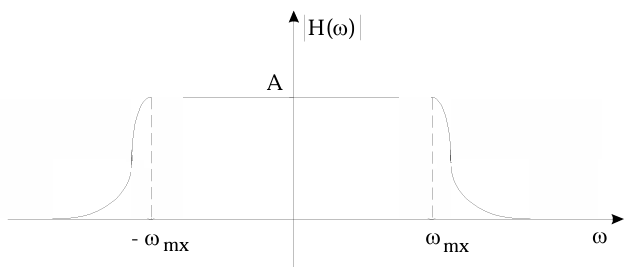
\includegraphics[scale = 0.5]{Spettro dei moduli di un filtro lineare.PNG}
    \end{figure}  
     
}


{
    \begin{figure}[h]
        \centering
        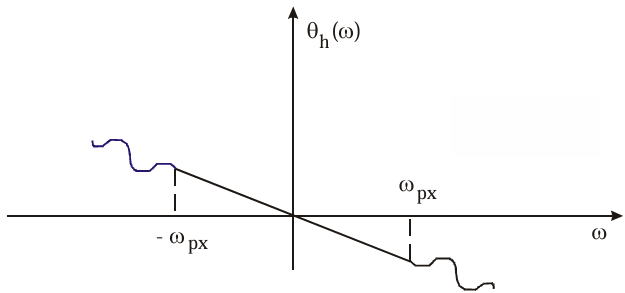
\includegraphics[scale = 0.5]{Spettro delle fasi di un filtro lineare.PNG}
    \end{figure}  
     
} 

\newpage  


Praticamente, tutti i mezzi trasmissivi utilizzati nei sistemi di comunicazione presentano 
un comportamento passa-basso, e dunque eliminano le componenti ad alta frequenza del segnale che li attraversa. \newline 

Le componenti ad alta frequenza sono responsabili delle transizioni veloci. \newline 

Quindi, il segnale filtrato è costretto ad assumere un andamento più "smussato". \newline 

Definiamo come dispersione il meccanismo di allargamento nel tempo del segnale. \newline 

Gli effetti della dispersione sono particolarmente dannosi nelle trasmissioni numeriche, 
dove il segnale trasmesso è costituito da una sequenza di impulsi. \newline 

{
    \begin{figure}[h]
        \centering
        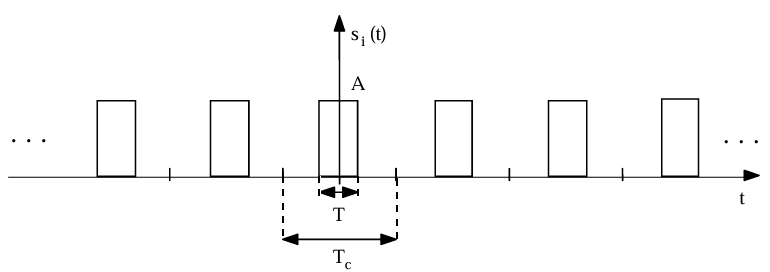
\includegraphics[scale = 0.75]{Treno di impulsi.PNG} 
        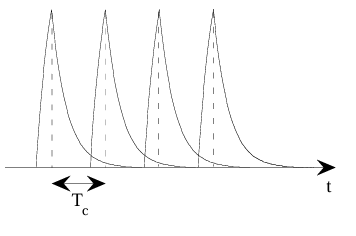
\includegraphics[scale = 0.75]{Treno di impulsi filtrato.PNG}
    \end{figure}  
     
}

Le due figure mostrano, in alto, il segnale di ingresso, in basso, il segnale filtrato. \newline 

Dalla figura del treno di impulsi filtrato, notiamo che la coda del generico impulso si sovrappone 
agli impulsi successivi, determinando il fenomeno denominato "interferenza di intersimbolo" (o ISI). \newline 

Oltre ai filtri passa-basso, esistono anche i filtri passa-alto, che, a differenza dei filtri passa-basso, 
fanno passare le frequenze ad alta frequenza, non lasciando passare le frequenze a bassa frequenza. \newline 

Nella realtà, questi filtri non esistono, sono un'astrazione puramente matematica. \newline 

Nella realtà, oltre ai filtri-passa basso, avremo i filtri passa-banda (che a sua volta sono formati 
da due filtri passa-basso) che, come dicono il nome, fanno passare le componenti in frequenza di una certa banda. \newline 

Generalmente, nei mezzi trasmissivi e negli apparati ad essi collegati, il canale di trasmissione, oltre 
a bloccare la componente continua, $\omega = 0$, elimina le componenti ad alta frequenza, $\omega > \omega_{px}$. \newline 

Dunque, la migliore modellazione di un sistema di comunicazione è quella di un filtraggio passa-banda. \newline 

\newpage 

\subsection{Distorsione non lineare} 

La proprietà di linearità di un dato sistema non è indipendete dal segnale di ingreso. \newline 

Il comportamento lineare vale sotto l'potesi di applicazione di (relativamente) piccoli segnali. \newline 

Quando l'ampiezza della sollecitazione diventa elevata, 
una descrizione accurata del sistema non può più prescindere dalle non linearità. \newline 

Quando l'ipotesi di piccoli segnali non può essere ritenuta valida, le non linearità devono 
essere introdotte nella descrizione del sistema e ne modificano significativamente la caratterizzazione. \newline 

Ci sono delle differenze rispetto alla distorsione lineare. \newline 

Il legame ingresso-uscita nel dominio del tempo non può più essere descritto da un integrale di convoluzione: 
è necessario specificare puntualmente il valore assunto dall'uscita in corrispondenza di un dato valore all'ingresso. \newline 

Supponendo che il legame sia instantaneo (sistema non lineare senza memoria), 
la caratteristica che lega il segnale di uscita y(t) a quello di ingresso x(t) può essere espressa come: 

{
    \Large 
    \begin{equation}
        y(t) = f[x(t)]
    \end{equation}
} 

dove f è una funzione generica non lineare. \newline 

Se f è una funzione non lineare, y(t) possiamo esprimerlo con lo sviluppo in serie di Mac-Laurin come: 

{
    \Large 
    \begin{equation}
        y(t) 
        =
        a_0 + a_1 x(t) + a_2 x^{2} (t) + a_3 x^{3} (t) + .... + a_k x^{k} (t) + ...
    \end{equation}
}

Se y(t) è composto dai coeffiecienti $a_0$ e/o $a_1$, allora possiamo dire che y(t) è legato 
linearmente da x(t), se y(t) è composto da coefficienti maggiori di uno, allora y(t) è legato 
da x(t) da una relazione non lineare. \newline 

A causa della loro non linearità, per i sistemi non lineari non è definibile una funzione di trasferimento. \newline 

Per i sistemi non lineari, dovremo svolgere k convoluzioni per quanti sono i coeffcienti dello sviluppo in serie di 
Mac-Laurin di y(t). \newline 

\newpage 

\subsection{Distorsione causata da percorsi multipli} 

Una trasmissione a percorsi multipli (in inglese Multipath) ha 
luogo quando il segnale trasmesso arriva al ricevitore seguendo due o più percorsi caratterizzati da ritardi differenti. \newline 

Uno schema di quello che succede, ad esempio, in una trasmissione radio: 

\begin{figure}[h]
    \centering
    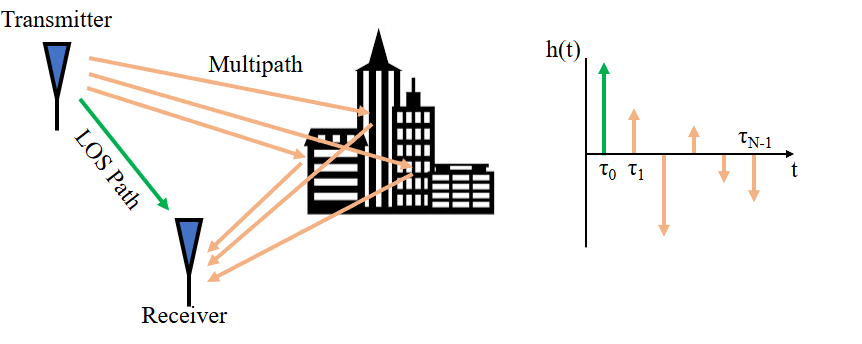
\includegraphics[scale = 0.6]{Multipath IRL.PNG}
\end{figure} 

In presenza di percorsi multipli, il canale può essere schematizzato mediante più canali in parallelo, ciascuno con differente attenuazione relativa e differente 
ritardo temporale. \newline 

{
    \begin{figure}[h]
        \centering
        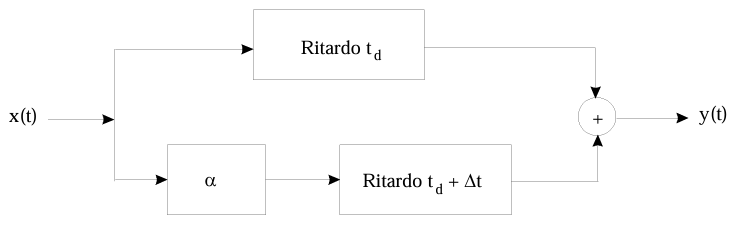
\includegraphics[scale = 1]{Esempio di multipath.PNG} 
    \end{figure}  
     
}

La seguente figura è un esempio di multipath con due soli percorsi: 
\begin{itemize}
    \item uno con guadagno unitario e ritardato di $t_d$ 
    \item l'altro con guadagno $\alpha$ e ritardato di $t_d + \Delta t$
\end{itemize}  

Tipicamente, $\alpha < 1$: in questo caso si tratta, propriamente, di un'attenuazione; 
se $\alpha > 1$ si tratta di amplificazione, me generalemente ciò non capita nel multipath. \newline  

Se consideriamo questo multipath, in frequenza, considerando i due cammini, avremo che: 

{
    \Large 
    \begin{equation}
        \begin{cases}
            H_1 (\omega) = e^{-\jmath \omega t_d} \\ 
            H_2 (\omega) = \alpha e^{-\jmath \omega (t_d + \Delta t)} 
        \end{cases}
    \end{equation}
} 

Quindi, la funzione di trasfermineto dell'intero sistema è: 

{
    \Large 
    \begin{equation}
        \begin{split}
            H(\omega) 
            &= 
            H_1 (\omega) + H_2 (\omega) 
            \\ 
            &= 
            e^{-\jmath \omega t_d} +  \alpha e^{-\jmath \omega (t_d + \Delta t)} 
            \\ 
            &= 
            e^{-\jmath \omega t_d} (1 + \alpha e^{-\jmath \omega \Delta t}) 
            \\
            {
                \small
                \text{Applicando la formula di Eulero }
            }
            &= 
            e^{-\jmath \omega t_d} 
            [1 + \alpha \cos(\omega \Delta t) - \jmath \alpha \sin(\omega \Delta t)] 
            \\ 
            &= 
            \sqrt{1 + \alpha ^{2} + 2 \alpha \cos(\omega \Delta t)} 
            \cdot 
            e^{-\jmath [\omega t_d + \arctan \frac{\alpha \sin(\omega \Delta t)}{1 + \alpha \cos(\omega \Delta t)}]}
        \end{split}
    \end{equation}
}

Si può concludere che la trasmissione multipath dà luogo ad una funzione di trasferimento non ideale (sia nell'ampiezza che nella fase) 
ed è quindi responsabile di una particolare distorsione lineare. \newline 

In quanto tale, tale distorsione può essere almeno parzialmente corretta con l'uso di equilizzatori. \newline 

{
    \begin{figure}[h]
        \centering
        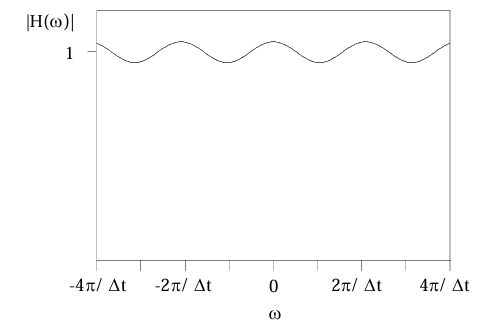
\includegraphics[scale = 0.5]{Esempio di multipath modulo.PNG}
        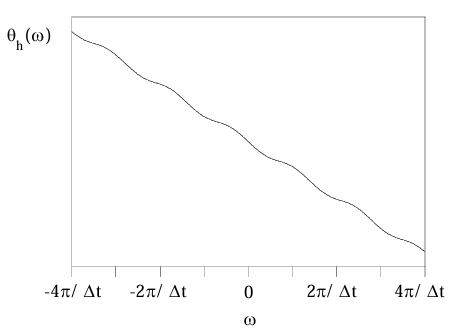
\includegraphics[scale = 0.5]{Esempio di multipath fase.PNG}  
    \end{figure}  
     
} 
\newpage 

\subsection{Canali con fading}

Fino ad ora abbiamo assunto le caratteristiche del canale costanti nel tempo. \newline 

Tuttavia, nella pratica e nella vita reale, molti canali di trasmissione presentano proprietà variabili nel tempo. \newline 

Il canale cambierà le sue proprietà nel tempo. \newline

Perciò, la funzione di trasferimento del canale varia a sua volta nel tempo in maniera aleatoria, causando attenuazione pure aleatorie 
(o random in inglese) del segnale. \newline 

Questo tipo di fenomeno è noto come fading. \newline 

\newpage 
.
\newpage
. 
\newpage

\chapter{Cenni sulla sintesi dei filtri analogici e filtri numerici}

\begin{figure}[h]
    \centering
    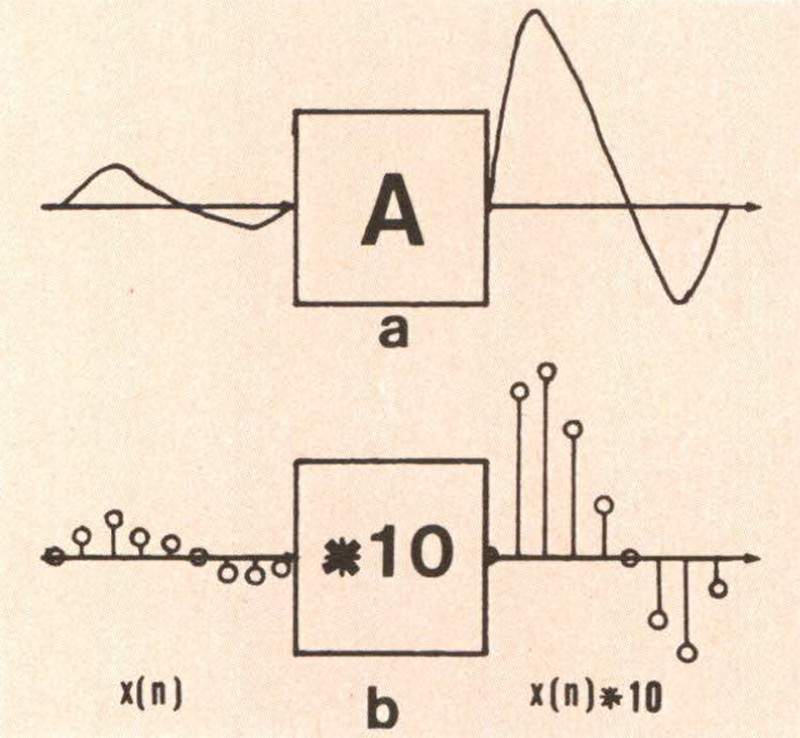
\includegraphics[scale = 0.5]{Filtro analogico e filtro numerico esempio.jpg}
\end{figure}  

\newpage 

\section{Sintesi di un filtro}

Idelmente, si progetta un filtro per eliminare parte del contenuto armonico di un segnale, 
lasciandone inalterata la porzione restante. \newline 

L'intervallo di frequenze del segnale in cui il filtro nominalmente non apporta delle modifiche  
prende il nome di banda passante del filtro. \newline 

Un filtro, in base al suo scopo, viene definito come: 

\begin{itemize}
    \item filtro passa-basso 
    \item filtro passa-alto 
    \item filtro passa-banda 
\end{itemize} 

Un filtro ideale dovrebbe essere caratterizzato da una funzione di trasferimento unitaria all'interno della banda passante, 
mentre la funzione di trasferimento dovrebbe essere identicamente nulla all'esterno della banda passante. \newline 

In altri termini, il filtro non dovrebbe attenuare le frequenze desiderate, 
mentre l'attenuazione dovrebbe essere infinita per quelle indesiderate. \newline 

Grazie alla definizione e spiegazione di cosa è un filtro, 
possiamo scrivere che è importante sia lo spettro di ampiezza della funzione di trasferimento 
che lo spettro di fase. \newline 

Idealmente, un filtro dovrebbe introdurre un ritardo costante su tutte le componenti armoniche entro la banda passante, 
e questo si traduce, notorialmente, in un andamento lineare della sua caratteristica di fase nello stesso intervallo 
di frequenze. \newline 

Il comportamento ideale, riguarda la transizione brusca da banda passante (in inglese pass band) 
a banda eliminata (stop band) può essere approssimato da un filtro reale. \newline 

La sintesi di un filtro comincia con l'assegnazione della cosiddetta "maschera" (mask) del suo spettro di ampiezza. \newline 

La maschera contiene le informazioni sul comportamento del filtro (quindi se è un filtro passa-alto, passa-basso, passa-banda) 
e le tolleranze ammissibili. \newline 

Siccome il comportamento ideale non portrà mai essere conseguito, si accettano i seguenti criteri: 

\begin{itemize}
    \item lo spettro di ampiezza (cioè il modulo della funzione di trasferimento) del filtro presenti una oscillazione (ripple) residua all'interno della banda passante 
    \item la regione di transizione da banda passante a banda eliminata abbia estensione non nulla 
    \item il comportamento in banda eliminata possa essere non ideale, con una oscillazione intorno allo zero, ovvero con una tendenza asintotica a zero 
\end{itemize}

La maschera del filtro, impostata in fase di progetto, specifica i margini di accettibilità delle non idealità elencate. \newline 

\newpage 

\subsection{Esempi di filtri passa-basso} 

\begin{figure}[h]
    \centering
    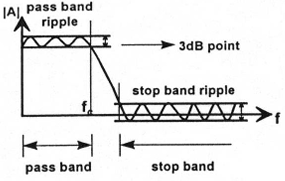
\includegraphics[scale = 1]{Sintesi di un filtro passa-basso.PNG}
\end{figure}  

Questo è un esempio di una maschera di un filtro passa-basso. \newline 

Possiamo notare che: 

\begin{itemize}
    \item il valore del guadagno in banda passante, idealmente dovrebbe essere uguale a uno, ma nella realtà può essere maggiore di 1 se il filtro amplifica o minore di 1 se il filtro attenua 
    \item la frequenza di taglio $f_c$ del filtro, definita come il valore di frequenza per cui il guadagno è sceso di $\frac{1}{\sqrt{2}} = 0.707$ volte il valore nominale all'interno della banda passante. \\ 
    In altri termini, considerando il guadagno del filtro $\abs{A_0}$ si ha dunque $\abs{H(f_c)} = \frac{A_0}{\sqrt{2}}$ o, usando i db, $\abs{H(f_c)}_{db} = \abs{A_0}_{db} - 3_{db}$ 
\end{itemize}

Un filtro passa-basso di questo tipo può essere sintetizzato, quindi progettato e fisicamente realizzato, assemblando insieme componenti resistivi, capacitivi e induttivi, 
scegliendo a priori la frequenza di taglio desiderata. \newline 

Ci sono diverse famiglie di filtri. \newline 

Un esempio di famiglia di filtri passa-basso sono i filtri di Butterworth. \newline 

L'andamento del modulo, per questa famiglia di filtri, è del tipo: 

{
    \Large 
    \begin{equation}
        \abs{H_n (f)} = \abs{A} = \frac{1}{\sqrt{1+(\frac{f}{f_c})^{2n}}}
    \end{equation}
}

dove n è un numero intero e indica l'ordine del filtro: il suo valore determina l'estensione della regione di transizione da banda passante a banda eliminata. \newline 

Di seguito, il modulo, la fase e la realizzazione di un filtro di Butterworth: 

\begin{figure}[h]
    \centering
    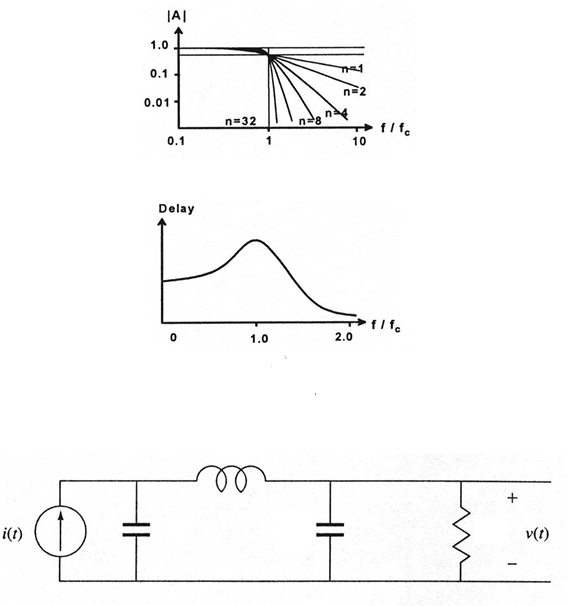
\includegraphics[scale = 1]{Realizzazione e progettazione di un filtro di Butterworth.PNG}
\end{figure}  

Un'altra famiglia di filtri passa-basso sono i filtri di Chebyshev. \newline 

Un filtro di Chebyshev è caratterizato da un andamento dello spettro di ampiezza esprimbile come : 

{
    \Large 
    \begin{equation}
        \abs{H_n (f)} = \frac{1}{\sqrt{1 + \varepsilon_p C_n ^{2} (\frac{f}{f_s})}}
    \end{equation}
} 

\newpage 

Di seguito, lo spettro delle ampiezze di due filtri Chebyshev: 

\begin{figure}[h]
    \centering
    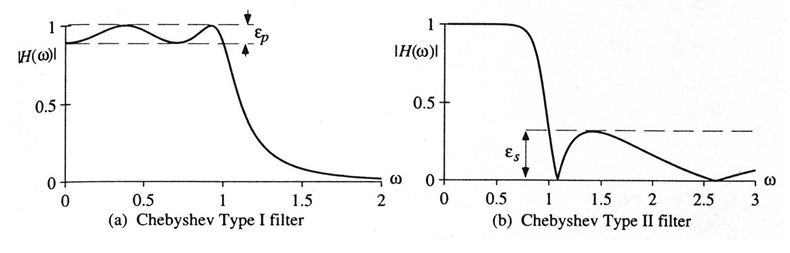
\includegraphics[scale = 1]{Filtri di Chebyshev di ordine 1 e 2.PNG}
\end{figure}  

Un'altra famiglia di filtri sono quelli di Bessel, il cui modulo è costante per tutte le frequenze, ma è molto utile per migliorare la fase. \newline 

\newpage 

\subsection{Esempi di filtri digitali} 

Se il segnale è digitale, quindi non è più analogico, avremo bisogno di filtri digitali, 
quindi non ci saranno più resistori, induttori e condensatori bensì effcienti programmi di calcolo 
chiamati software packages. \newline 

I filtri digitali prendono il nome anche di filtri numerici (in inglese digital filter). \newline 

Un filtro digitale è costituito da: 

\begin{itemize}
    \item x[n], il segnale di ingresso, è costituito da una serie di campioni discreti, estratti da una forma continua alla frequenza di campionamento $f_s$ in cui ogni $x[n_i]$ è contenuto in un regostro
    \item Blocchi $z^{-1}$ che rappresentano un ritardo di simbolo, o periodo di campionamento $T_s = \frac{1}{f_s}$ 
    \item tap, che sono gli elementi di ritardo 
    \item weight, o pesi in italiano, sono i coefficienti che moltiplicano le uscite dei tap 
    \item sommatori (in inglese summing function) che sommano le uscite dei tap pesate dai wieght
\end{itemize} 

Un esempio di filtro digitale: 

\begin{figure}[h]
    \centering
    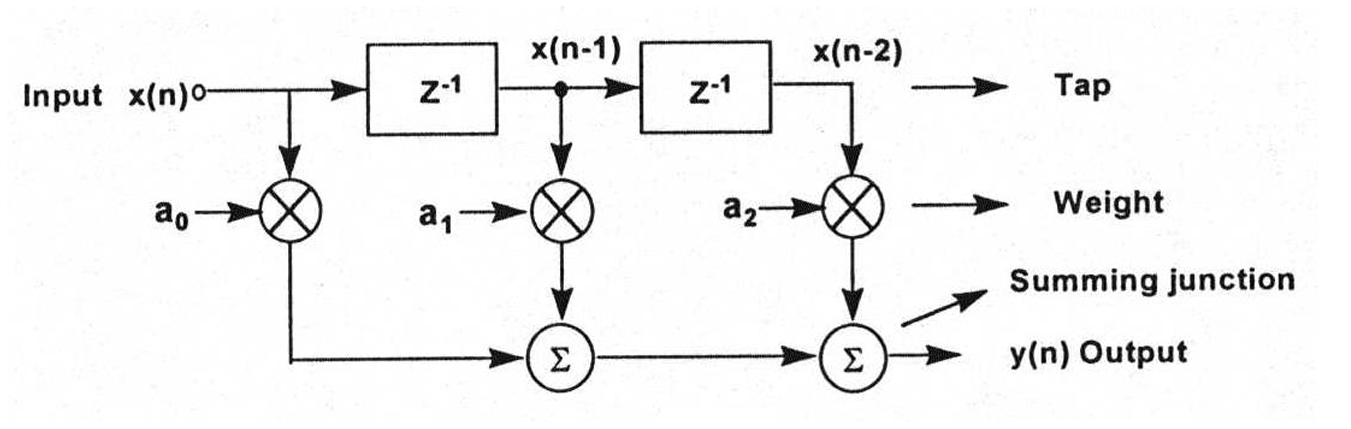
\includegraphics[scale = 0.55]{Esempio di filtro digitale.PNG}
\end{figure}  

La funzione di uscita del filtro di esempio è: 

{
    \Large 
    \begin{equation}
        y[n] = a_0 x[n] + a_1 x[n -1] + a_2 x[n-2]
    \end{equation}
}

Come nel caso analogico, se il filtro è lineare, possiamo esprimere l'uscita di un filtro con la sua risposta impulsiva: 

{
    \Large 
    \begin{equation}
        y[n] = \sum_{\kappa = -\infty}^{\infty} x[n] h[n-k]
    \end{equation}
}

Questa equazione è la convoluzione in digitale, in cui x[n] è la seguenza di ingresso e h[n] è la risposta impulsiva. \newline  

In base alla risposta impulsiva del filtro, possiamo distinguere due categorie di filtri: 

\begin{itemize}
    \item i FIR, Finite Impulse Response 
    \item gli IIR, Infinite Impulse Response 
\end{itemize}

I FIR hanno questo nome perchè la loro risposta impulsiva è finita, quindi la loro uscita è del tipo: 

{
    \Large 
    \begin{equation}
        y[n] = \sum_{\kappa = 0}^{M} b_\kappa x[n - \kappa]
    \end{equation}
}


La loro risposta impulsiva è del tipo: 

{
    \Large 
    \begin{equation}
        h[n] = \sum_{\kappa = 0}^{M} b_\kappa \delta[n - \kappa] = 
        \begin{cases}
            b_n \text{ se } 0 \leq n \leq M \\ 
            0 \text{ altrimenti }
        \end{cases}
    \end{equation}
}

Un filtro in cui la risposta dipende dall'uscita negli istanti precedenti è un filtro ricorsivo, o anche detto IIR. \newline 


I filtri IIR sono, in linea di principio, più efficienti rispetto ai filtri FIR perchè hanno bisogno di meno tap per
avere lo stesso roll-off rate. \newline 

In certi casi, si preferiscono i filtri FIR grazie alla loro caratteristica di essere, per definizione, sempre stabili. \newline 

In generale, maggiori sono i registri, maggiore sarà il tempo di elaborazione. \newline 

\newpage 
. 
\newpage
. 
\newpage 
\chapter{Teorema del campionamento} 

\begin{figure}[h]
    \centering
    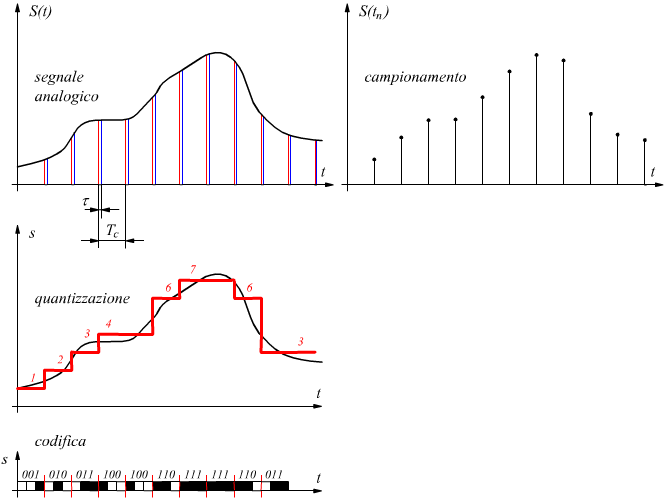
\includegraphics[scale = 0.6]{Campionamento segnale.png}
\end{figure}  

\newpage 

\section{Cosa è il campionamento e quali segnali soddisfano questo tipo di rappresentazione} 

Come la trasformata di Forurier, anche il teorema del campionamento può essere visto come una 
possibile rappresentazione del segnale. \newline 

Il campionamento non modifica il dominio del segnale s(t), quindi il dominio del segnale campionato 
rimane quello dei tempi. \newline 

I segnali che possono essere campionati sono quelli limitati in banda, con banda compresa (in pulsazione) tra 
$-2\pi B$ e $2\pi B$. \newline 

Se consideriamo B costante, appartengono alla classe i segnali che non vengono alterati nel transito 
attraverso un filtro passa-basso ideale con banda $2 \pi B$. \newline 

Un esempio grafico di un segnale campionabile: 

\begin{figure}[h]
    \centering
    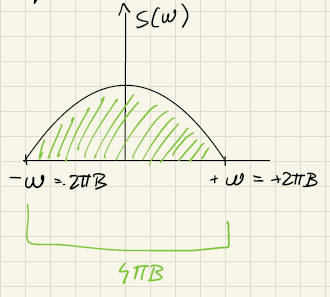
\includegraphics[scale = 0.6]{Segnale campionabile schema.PNG}
\end{figure}  

Il teorema del campionamento stabilisce che la conoscenza del segnale s(t) è del tutto 
equivalente alla conoscenza dei suoi campioni $s(k T_c)$, con k variabile intera, 
ottenuti calcolando s(t) per $t=kT_c$. \newline 

$T_c$ prende il nome di intervallo (o tempo) di campionamento. \newline 

Il suo inverso 
{
    \Large 
    \begin{equation}
        f_c = \frac{1}{T_c}    
    \end{equation}
}

è la frequenza di campionamento e rappresenta il numero di campioni del segnale per unità di tempo 
che è necessario considerare ai fini della rappresentazione. \newline 

Quindi, grazie a questo teorema, conoscere i campioni ogni $T_c$ è come conoscere tutto s(t) continuo. \newline 

Come ogni rappresentazione, non solo è necessaria la procedura per definire i campione dal segnale s(t), 
ma è anche necessaria la procedura inversa. \newline 

Consideriamo il segnale s(t) e la sua trasformata di Forurier $S(\omega)$. \newline 

Possiamo vedere $S(\omega)$ come alla rappresentazione elementare (all'interno di un periodo) di un segnale periodico in $\omega$ con periodo pari a $4\pi B$ 
in cui il segnale è centrato in $\omega = 0$. \newline 

Il segnale poi, viene periodicizzato nello spettro del segnale, proprietà molto importante nel campionamento. \newline 

In quanto periodica, la funzione così ottenuta può infatti essere sviluppata in serie di Fourier: 
rispetto alla notazione classica (in cui il segnale che viene sviluppato è una funzione del tempo) 
occorre sostituire t con $\omega$ e tener conto del fatto che il periodo vale $4 \pi B$. \newline 

{
    \Large 
    \begin{equation}
        S(\omega) 
        = 
        \frac{1}{\sqrt{4\pi B}} 
        \sum_{k = -\infty}^{+ \infty} 
        c_k e^{\frac{\jmath k \omega}{2B}}
    \end{equation}
}

{
    \Large 
    \begin{equation}
        c_k 
        = 
        \frac{1}{\sqrt{4 \pi B}} 
        \int_{-2 \pi B}^{2 \pi B}
        S(\omega) e^{-\frac{\jmath k \omega}{2B}} 
        d\omega
    \end{equation}
}

\newpage 

\subsection{Dimostrazione del Teorema del campionamnto}

Il segnale s(t) può essere espresso come anti-trasformata di $S(\omega)$, cioè: 

{
    \Large 
    \begin{equation}
        s(t) 
        = 
        \frac{1}{2 \pi} 
        \int_{-2\pi B}^{2\pi B} 
        S(\omega) e^{\jmath \omega t} 
        d\omega
    \end{equation}
}

Siccome il segnale s(t) è limitato in banda, risulta che: 

{
    \Large 
    \begin{equation}
        c_k 
        = 
        \sqrt{\frac{\pi}{B}}
        s(-\frac{k}{2B})
    \end{equation}
}

Sapendo che: 

{
    \Large 
    \begin{equation}
        T_c 
        = 
        \frac{1}{2B}
    \end{equation}
}

possiamo scrivere: 

{
    \Large 
    \begin{equation}
        c_k = \sqrt{\frac{\pi}{B}} s(-k T_c)
    \end{equation}
}

Questa ultima equazione esprime esplicitamente il teorema del campionamento. \newline 

Se infatti è vero che la conoscenza dei coeffiecienti $c_k$ è equivalente alla conoscenza della funzione 
$S(\omega)$ e quindi di s(t), questa ultima equazione ci dimostra che questi coefficienti possono essere determinati 
campionando il segnale s(t) in corrispondenza di multipli di $T_c$. \newline 

Un segnale limitato in banda non è necessariamente descritto dall'infinità non numerabili di valori 
che esso assume in ciascuno dei possibili istanti distinti nel tempo; 
per la sua completa conoscenza è sufficiente la determinazione dei valori che esso assume in corrispondenza di tutti e soli gli 
instanti multipli di $\frac{1}{2B}$. \newline 

\newpage 

\section{Ricostruzione del segnale s(t) partendo dai coefficienti} 

Partendo dalla definizione di segnale in $\omega$: 

{
    \Large 
    \begin{equation}
        S(\omega) 
        = 
        \frac{1}{\sqrt{4\pi B}} 
        \int_{k = -\infty}^{+ \infty} 
        c_k e^{\frac{\jmath k \omega}{2B}}
    \end{equation}
}

e sapendo che $c_k$, per un segnale limitato in banda, vale: 

{
    \Large 
    \begin{equation}
        c_k = \sqrt{\frac{\pi}{B}} s(-k T_c)
    \end{equation}
}

possiamo scrivere che $S(\omega)$ diventa: 

{
    \Large 
    \begin{equation}
        S(\omega) 
        = 
        \sum_{k = -\infty}^{+ \infty}
        \frac{1}{2B}
        s(-k T_c) e^{\jmath k \omega T_c}
    \end{equation}
}
Considerando solo l'intervallo di frequenze $[-2 \pi B, 2 \pi B]$ in cui è allocato il 
segnale s(t) e sostituendo -k con k, avremo che: 

{
    \Large 
    \begin{equation}
        S(\omega) 
        = 
        \sum_{k = -\infty}^{\infty} 
        \frac{1}{2B}
        s(kT_c) e^{-\jmath k \omega T_c}
        \text{ in } 
        -2\pi B \leq \omega \leq 2\pi B
    \end{equation}
}

Anti-trasformando $S(\omega)$, abbiamo che: 

{
    \Large 
    \begin{equation}
        \sum_{k = - \infty}^{+\infty} 
        s(kT_c) \frac{\sin[2\pi B(t-kT_c)]}{2 \pi B(t - kT_c)}
    \end{equation}
}

Siccome $\frac{\sin[2\pi B(t-kT_c)]}{2 \pi B(t - kT_c)}$, che prende il nome di funzione sinc, 
che ha massimo uguale a 1 in $t=kT_c$, prende il nome di funzione di campionamento. \newline 

Al variare di k, le funzione di campionamento che hanno la stessa struttura qualunque sia il segnale da rapppresentare, 
sono tra loro ortogonali. \newline 

Si hanno dunque condizioni analoghe a quelle dei segnali con sviluppo in serie di Forurier.\newline 

I campioni del segnale prendono dunque il posto dei coefficienti dello sviluppo in serie di Forurier. \newline 

\newpage 

\section{Dualità tempo-frequenza nel campionamento} 

Un'ulteriore considerazione riguardo il valore di $f_c$ è che, dalla definizione di $f_c$ e la relazione con B, abbiamo che: 

{
    \Large 
    \begin{equation}
        f_c = \frac{1}{T_c} = \frac{1}{\frac{1}{2B}} = 2B 
    \end{equation}
}

Quindi: 

{
    \Large 
    \begin{equation}
        f_c \geq 2B
    \end{equation}
}


All'aumentare di B, anche $f_c$ aumenta, tanto che al limite, per $B \rightarrow \infty$, 
il campionamento dovrebbe considerare tutti i possibili istanti temporali. \newline 

\newpage 

\section{Tipi di campionamento} 

In questa sezione analizzeremo quattro tipi di campionamento: 

\begin{itemize}
    \item Campionamento ideale 
    \item Campionamento naturale 
    \item Campionamento istantaneo 
    \item Campionamento di segnali passa-banda 
\end{itemize}

\newpage 

\subsection{Campionamento ideale}

Per campionamento ideale si intende il campionamento di un segnale utilizzando il 
famoso impulso matematico (Delta di Dirac), la quale ha durata infinitesima, ma ampiezza corrispondente infinita. \newline 

Consideriamo una successione di impulsi matematici: 

{
    \Large 
    \begin{equation}
        s_p 
        = 
        \sum_{k = -\infty}^{\infty} 
        \delta (t - k T_c)
    \end{equation}
}

Moltiplicando $s_p$ per s(t), possiamo svolgere un campionamento ideale. \newline 

Il segnale campionato in modo ideale sarà: 

{
    \Large 
    \begin{equation}
        \begin{split}
            s_c (t) 
            &= 
            s(t) \cdot s_p (t) 
            \\ 
            &= 
            s(t) \cdot \sum_{k = -\infty}^{\infty} \delta (t - k T_c)
            \\ 
            &= 
            \sum_{k = -\infty}^{\infty} s(k T_c) \delta (t - k T_c)
        \end{split} 
    \end{equation}
}

Avendo a che fare con una Delta di Dirac, nella realtà non riusciremo mai a realizzare un campionamento ideale. \newline 

Andando nel dominio in $\omega$, avremo che la successione di impulsi matematici $s_p (t)$ sarà: 

{
    \Large 
    \begin{equation}
        S_p (\omega) 
        = 
        \omega_c \sum_{k = - \infty}^{+ \infty} \delta (\omega - k \omega_c)    
    \end{equation}
}

in cui: 

{
    \Large 
    \begin{equation}
        \omega_c = 2\pi f_c = \frac{2\pi}{T_c}
    \end{equation}
}

Quindi, la trasformata di Fourier della sequenza di impulsi matematici distanziati nel tempo di $T_c$ è dunque, 
a sua volta, una sequenza di impulsi matematici distanziati in pulsazione di $\omega_c$. \newline 

Ricordando la proprietà della delta di Dirac, in cui la convoluzione con una funzione generica restituisce la funzione stessa centrata 
dove era posizionata la delta di Dirac, si può concludere che: 

{
    \Large 
    \begin{equation}
        \begin{split}
            S_c (\omega) 
            &= 
            \frac{\omega_c}{2 \pi} 
            \sum_{k = - \infty}^{ + \infty} 
            S(\omega - k \omega_c) 
            \\ 
            &= 
            \frac{1}{T_c} 
            \sum_{k = - \infty}^{ + \infty} 
            S(\omega - k \omega_c) 
        \end{split}
    \end{equation}
} 

Questi schemi possono essere utili per visualizzare le equazioni: 

\begin{figure}[h]
    \centering
    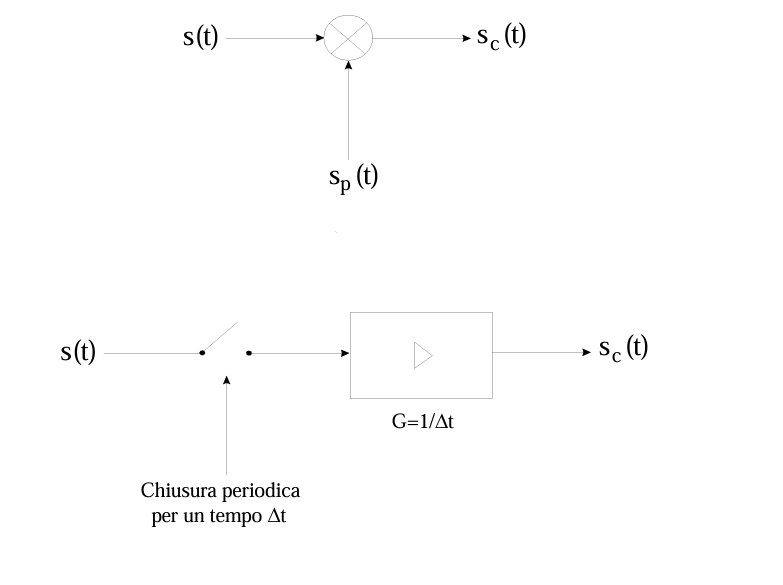
\includegraphics[scale = 0.6]{Campionamento ideale.PNG}
\end{figure}  

\newpage 

Ora facciamo lo step inverso. \newline 

Partendo dai campioni, possiamo riottenere il segnale: per fare ciò, ci serve un filtro passa-basso. \newline 

Lo schema generale del sistema diventa: 

\begin{figure}[h]
    \centering
    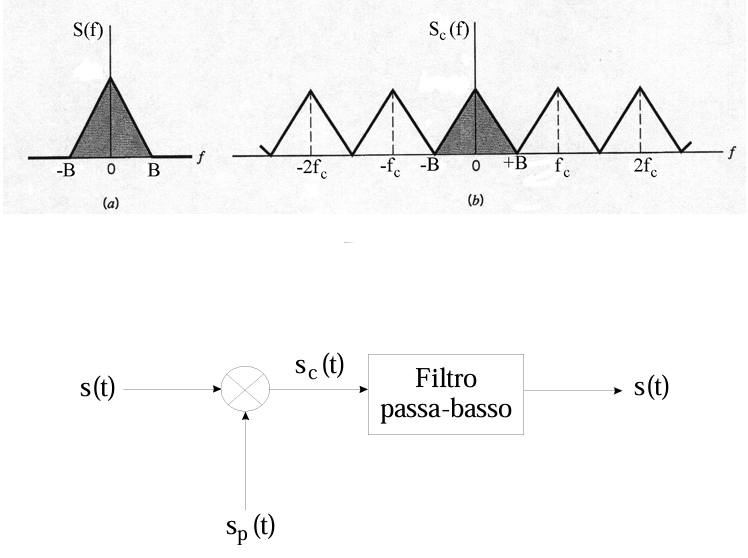
\includegraphics[scale = 0.6]{Dai campioni ideali al segnale.PNG}
\end{figure}  



Ponendo: 

{
    \Large 
    \begin{equation}
        f_c = 2B
    \end{equation}
} 

ci permette di non modificare il segnale originale senza avere distorsione. \newline 

Se invece: 

{
    \Large 
    \begin{equation}
        f_c < 2B
    \end{equation}
}

si sta svolgendo un sottocampionamento (undersampling in inglese). \newline 

Sottocampionando il segnale, questo ultimo avrà delle distorsioni, quindi degli effetti non lineari. \newline 

Un esempio di un sottocampionamento: 

\begin{figure}[h]
    \centering
    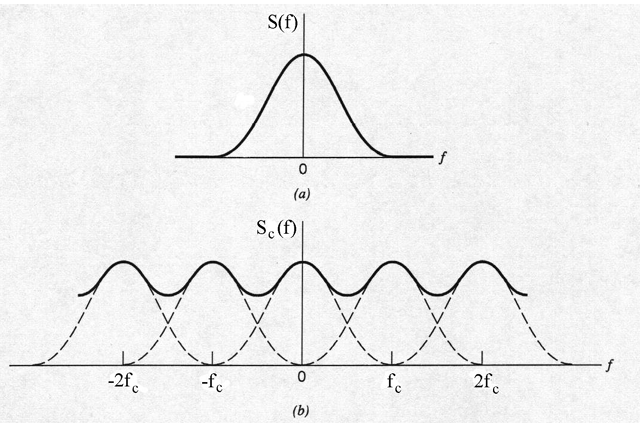
\includegraphics[scale = 0.6]{Esempio di sotto-campionamento.PNG}
\end{figure}  

\newpage 

Se invece si sovra-campiona, quindi: 

{
    \Large 
    \begin{equation}
        f_c > 2B
    \end{equation}
}

si sta sovracampionando (in inglese oversampling) il segnale. \newline 

L'assunzione di una frequenza di campionamento $f_c$ maggiore di quella strettamente necessaria, 
non altera le prestazioni del campionamento, anzi, ne semplifica l'implementazione pratica. \newline 

La condizione: 

{
    \Large 
    \begin{equation}
        f_c \geq 2B
    \end{equation}
} 

prende il nome di condizione di Nyquist. \newline 

Un esempio di sovra-campionamento: 

\begin{figure}[h]
    \centering
    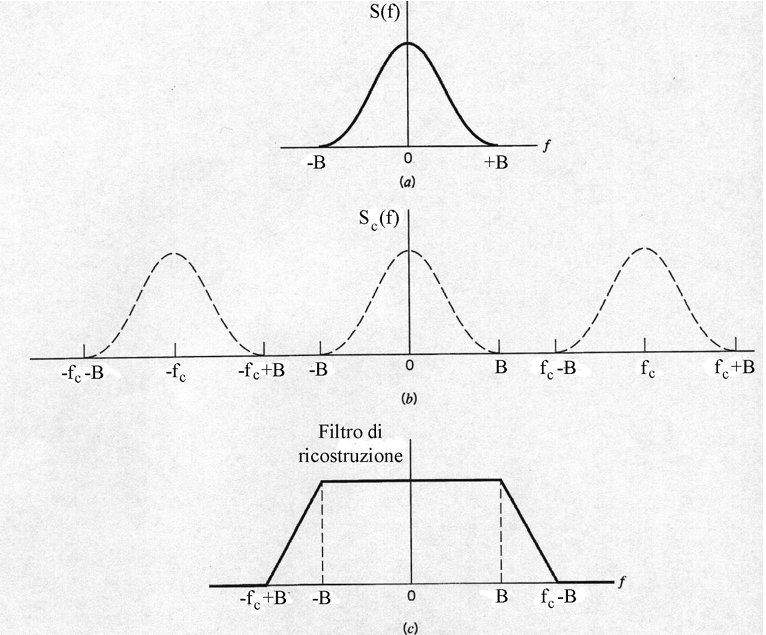
\includegraphics[scale = 0.6]{Esempio di segnale sovracampionato.PNG}
\end{figure}  

\newpage 

\subsection{Campionamento naturale} 

L'idealità dello schema di campionamento ideale sta nella impossibilità di utilizzare 
come funzione campionante una successione di Delta di Dirac. \newline 

Considerando questo sistema: 

\begin{figure}[h]
    \centering
    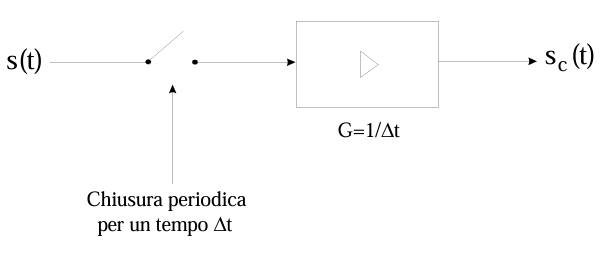
\includegraphics[scale = 0.6]{Campionamento naturale.PNG}
\end{figure}  

e $\Delta t$ un tempo infinitesimo, allora non avremo più una successione di impulsi, bensì 
una successione di impulsi rettangolari con seguente funzione: 

{
    \Large 
    \begin{equation}
        s_p (t) 
        = 
        \sum_{k= -\infty}^{+\infty}
        s_l (t- k T_c)
    \end{equation}
}

in cui $s_l (t)$ è l'impulso rettangolare unitario: 

{
    \Large 
    \begin{equation}
        s_l (t) 
        = 
        \begin{cases}
            1 \text{ se } \abs{t} \leq \frac{\Delta t}{2} \\ 
            0 \text{ se } \abs{t} > \frac{\Delta t}{2} 
        \end{cases}
    \end{equation}
}

Quando il segnale $s_p (t)$ è moltiplicao per s(t), il segnale campionato segue esattamente l'andamento del segnale in ingresso, 
ma limitatamente agli intervalli, periodici, di durata $\Delta t$. \newline 

Dal punto di vista grafico, il campionamento naturale di un segnale sarà: 

\begin{figure}[h]
    \centering
    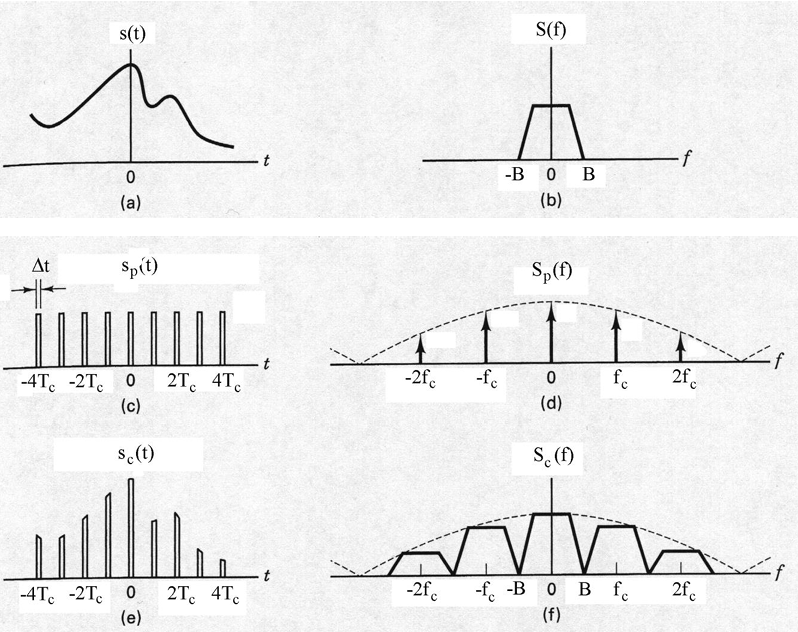
\includegraphics[scale = 0.7]{Segnale con campionamento naturale.PNG}
\end{figure}  

Più che una conoscenza puntuale del segnale s(t), si può qui parlare di conoscenza "intervallata" in porzioni di tempo 
significativamente più piccole del dominio originale. \newline 

Rispetto al caso ideale, si ha una ridondanza di informazione. \newline 

L'espressione matematica del segnale campionato, è, in questo caso, data da: 

{
    \Large 
    \begin{equation}
        \begin{split}
            s_c (t)
            &= 
            s(t) \cdot s_p (t)
            \\ 
            &= s(t) \sum_{k = -\infty}^{+ \infty} s_l (t - kT_c) 
        \end{split}
    \end{equation}
}

Il segnale campionante $s_p (t)$ è periodico, e dunque la sua trasformata vale: 

{
    \Large 
    \begin{equation}
        \begin{split}
            S_p (\omega) 
            &= 
            \omega_c 
            \sum_{k = -\infty}^{+ \infty}
            S_l (\omega) \delta (\omega - k \omega_c)
            \\ 
            &= 
            \omega_c 
            \sum_{k = -\infty}^{+ \infty}
            \Delta t 
            \frac{\sin(\omega \frac{\Delta t}{2})}{\omega \frac{\Delta t}{2}} 
            \delta (\omega - k \omega_c) 
            \\ 
            &= 
            \omega_c 
            \sum_{k = -\infty}^{+ \infty}
            \Delta t 
            \frac{\sin(k \omega_c \frac{\Delta t}{2})}{k \omega_c \frac{\Delta t}{2}} 
            \delta (\omega - k \omega_c)
        \end{split}
    \end{equation}
}

Considerando $S_l (\omega)$ la trasformata di Fourier dell'impulso rettangolare, il segnale campionato sarà del tipo: 

{
    \Large 
    \begin{equation}
        S_c (\omega) 
        = 
        \frac{\Delta t}{T_c} 
        \sum_{k = -\infty}^{+ \infty} 
        \frac{\sin (k \omega_c \frac{\Delta t}{2})}{k \omega_c \frac{\Delta t}{2}} 
        S(\omega - k \omega_c)
    \end{equation}
}

A meno del fattore $\Delta t$ e il conributo per $k = 0$, 
le due repliche sono moltiplicate per $\frac{\sin (k \omega_c \frac{\Delta t}{2})}{k \omega_c \frac{\Delta t}{2}} < 1$, 
ma mantengono esattamente la forma dello spettro originale, e dunque non sono distorte. \newline 

\newpage 

\subsection{Campionamento istantaneo}

Un primo, ma importante, passo verso la numerizzazione del segnale si ottiene considerando il campionamento istantaneo. \newline 

Un esempio di campionamento istantaneo: 

\begin{figure}[h]
    \centering
    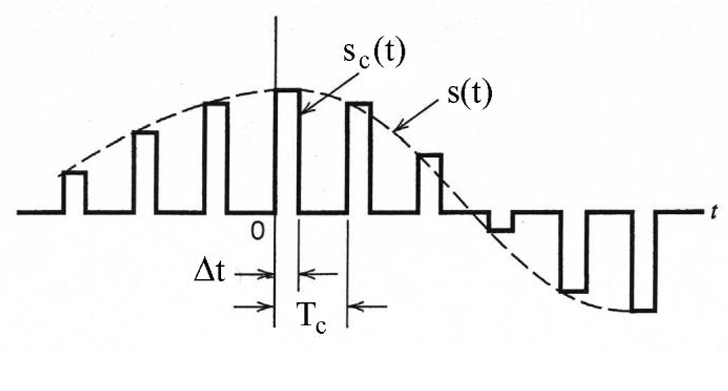
\includegraphics[scale = 0.6]{Esempio di segnale con campionamento istantaneo.PNG}
\end{figure}  

Rispetto al campionamento naturale, all'interno degli intervalli di durata $\Delta t$, 
il segnale campionato non segue il segnale originale, ma conserva il valore negli istanti di campionamento. \newline 

Quindi, il segnale con campionamento istantaneo è un segnale distorto, in altre parole, il segnale 
campionato in modo istantaneo è diverso da quello originale. \newline 

In pratica, il valore campionarto nell'istante $t = kT_c$ viene prolungato per l'intero intervallo $kT_c \leq t \leq kT_c + \Delta t$. \newline 

Un esempio di circuito per un campionamento istantaneo è quello del sample and hold (in italiano campionamento e tenuta). 

\begin{figure}[h]
    \centering
    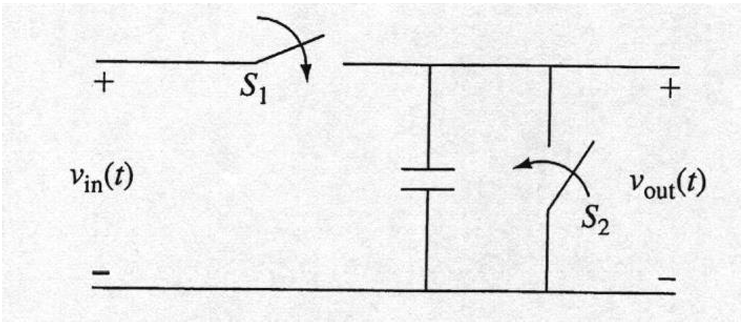
\includegraphics[scale = 0.6]{Circuito Sample and hold.PNG}
\end{figure} 

Il fatto che negli intervalli di durata $\Delta t$ il segnale campionato non segua l'andamento di s(t) ma venga forzato a rimanere costante, introduce evidentemente 
un'alternazione che è ragionevole pensare possa tradursi in una distorsione del segnale ricostruito. \newline 

Per valutare l'entità di questa distorsione, scriviamo l'entità di questa distorsione, scriviamo l'espressione del segnale campionato nel cao di campionamento istantaneo: 

{
    \Large 
    \begin{equation}
        s_c (t) 
        = 
        \sum_{k = - \infty}^{\infty}
        s(kT_c) 
        s_l (t-kT_c)
    \end{equation}
} 

Utilizzando la proprietà della convoluzione, $s_c (t)$ possiamo riscriverla come: 

{
    \Large 
    \begin{equation}
        s_c (t) = s_l \otimes s(t) \sum_{k = -\infty}^{\infty} \delta (t - k T_c)
    \end{equation}
}

dove: 

{
    \Large 
    \begin{equation}
        s_l (t) \otimes \delta(t - kT_c) = s_l (t - kT_c)
    \end{equation}
}

Applicando la proprietà della convoluzione e quella del prodotto, la trasformata di Fourier 
di $s_c (t)$ potrà riscriversi come: 

{
    \Large 
    \begin{equation}
        \begin{split}
            S_c (\omega) 
            &=
            \frac{1}{T_c} S_l (\omega) 
            \sum_{k = - \infty}^{\infty} 
            S(\omega -k \omega_c) 
            \\ 
            &=
            \frac{\Delta t}{T_c} 
            \frac{\sin(\omega \frac{\Delta t}{2})}{\omega \frac{\Delta t}{2}} 
            \sum_{k = -\infty}^{\infty} 
            S(\omega - k\omega_c)
        \end{split}
    \end{equation}
}

Confronta i tre casi di campionamento in $\omega$: \newline 

\textbf{Campionamento istantaneo}

{
    \Large 
    \begin{equation}
        S_c (\omega) = 
        \frac{\Delta t}{T_c} 
        \frac{\sin(\omega \frac{\Delta t}{2})}{\omega \frac{\Delta t}{2}} 
        \sum_{k = -\infty}^{\infty} 
        S(\omega - k\omega_c)
    \end{equation}
}

\textbf{Campionamento natuale}

{
    \Large 
    \begin{equation}
        S_c (\omega) = 
        \frac{\Delta t}{T_c} 
        \frac{\sin(\omega \frac{\Delta t}{2})}{k \omega_c \frac{\Delta t}{2}} 
        \sum_{k = -\infty}^{\infty} 
        S(\omega - k\omega_c)
    \end{equation}
}

\textbf{Campionamento ideale} 

{
    \Large 
    \begin{equation}
        S_c (\omega) = 
        \frac{1}{T_c} 
        \sum_{k = -\infty}^{\infty}
        S(\omega - k\omega_c)
    \end{equation}
}

notiamo che le singole repliche dello spettro del segnale originale sono, 
in questo caso, moltiplicate non per un valore costante (come avviene nel caso di campionamento naturale) 
ma, nel campionamento instantaneo, lo spettro segnale viene moltiplicato per una funzione in $\omega$. \newline 

In particolare, il filtro passa-basso di ricostruzione che isola la replica centrata nell'origine, 
darà in uscita un segnale $s^{'} (t)$ il cui spettro vale: 

{
    \Large 
    \begin{equation}
        S^{'} (\omega) = 
        \frac{\Delta t}{T_c} 
        \frac{\sin(\omega \frac{\Delta t}{2})}{\omega \frac{\Delta t}{2}} 
        S(\omega)
    \end{equation}
}

Si tratta dunque dello spettro di $S(\omega)$ moltiplicato per la funzione $sinc(\omega \frac{\Delta t}{2})$. 

Quindi, per riassumere, contrariamente agli altri tipi di campionamento, si avrà che: 

{
    \Large 
    \begin{equation}
        s^{'} (t) \neq s(t)
    \end{equation}
}

Un esempio dello spettro tra il campionamento ideale e campionamento istantaneo: 

\begin{figure}[h]
    \centering
    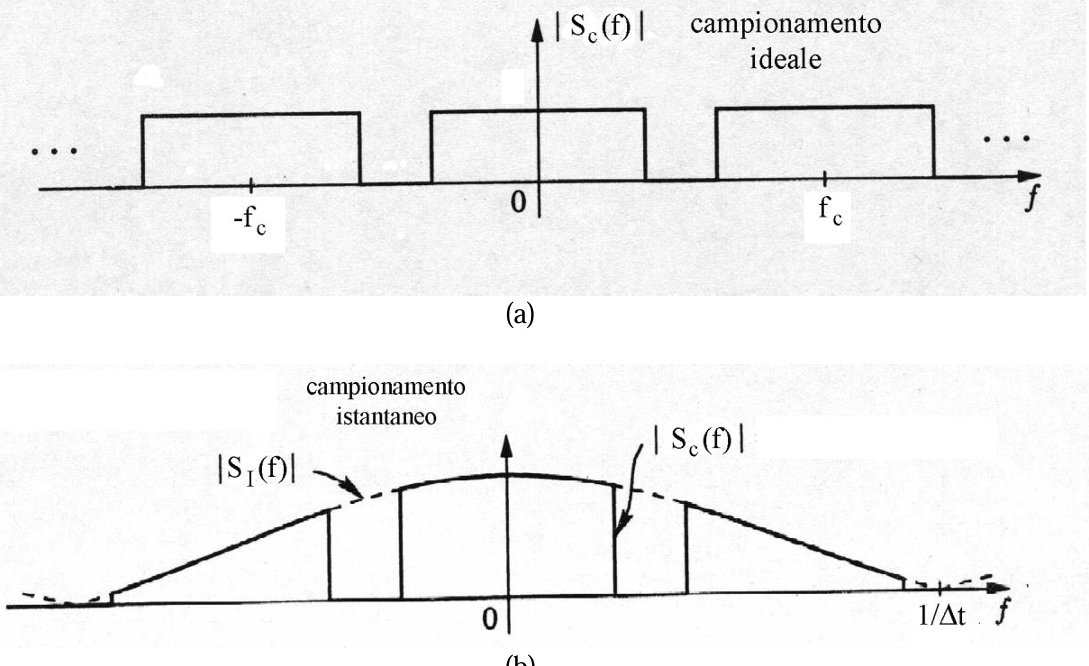
\includegraphics[scale = 0.6]{Differenze tra campionamento ideale e campionamento istantaneo.PNG}
\end{figure} 

\newpage 

Da questo confronto, possiamo svolgere due considerazioni. \newline

La prima considerazione da svolgere è che l'entità della distorsione è legata al valore di $\Delta t$. \newline 

Consideriamo il rapporto tra $\abs{S^{'} (\omega)}$ e $\abs{S(\omega)}$: 

{
    \Large 
    \begin{equation}
        \abs{\frac{S^{'} (\omega)}{S(\omega)}}
        = 
        \frac{\Delta t}{T_c}
        \abs{\frac{\sin(\omega \frac{\Delta t}{2})}{\omega \frac{\Delta t}{2}}} 
    \end{equation}
}

Di conseguenza, in $\omega = 0$: 

{
    \Large 
    \begin{equation}
        \left|\frac{S^{'} (\omega)}{S(\omega)} \right|_{\omega = 0} 
        = 
        \frac{\Delta t}{T_c}
    \end{equation}
} 

e 

{
    \Large 
    \begin{equation}
        \begin{split}
            \left|\frac{S^{'} (\omega)}{S(\omega)} \right|_{\omega = 2 \pi B} 
            &= 
            \frac{\Delta t}{T_c} 
            \abs{\frac{\sin(\pi B \Delta t)}{\pi B \Delta t}} 
            \\ 
            &= 
            \frac{2}{\pi} 
            \sin(\frac{\pi}{2} \frac{\Delta t}{T_c})
        \end{split}        
    \end{equation}

}

dove: 

{
    \Large 
    \begin{equation}
        B = \frac{1}{2 T_c} 
    \end{equation}
}

e 

{
    \Large 
    \begin{equation}
        \frac{\Delta t}{T_c} < 1        
    \end{equation}
}

Se consideriamo il rapporto tra i due rapporti di $S^{'}(\omega)$ e $S(\omega)$: 

{
    \Large 
    \begin{equation}
        \frac{\left|\frac{S^{'} (\omega)}{S(\omega)} \right|_{\omega = 2 \pi B}}{\left|\frac{S^{'} (\omega)}{S(\omega)} \right|_{\omega = 0}} 
        = 
        \frac{\sin(\frac{\pi}{2} \frac{\Delta t}{T_c})}{\frac{\pi}{2} \frac{\Delta t}{T_c}}
    \end{equation}
}

Se: 

{
    \Large 
    \begin{equation}
        \frac{\left|\frac{S^{'} (\omega)}{S(\omega)} \right|_{\omega = 2 \pi B}}{\left|\frac{S^{'} (\omega)}{S(\omega)} \right|_{\omega = 0}} 
        = 
        1  
    \end{equation}
}

la distorsione sarebbe nulla all'interno della banda del segnale. \newline 

Quanto minore è il rapporto $\frac{\Delta t}{T_c}$, tanto minore risulta la distorsione (si parla di effetto finestra). \newline 

Per alcune applicazioni un valore di $\frac{\Delta t}{T_c} < 0.1$ è già sufficiente per garantire distorsione trascurabile. \newline 


Un'altra considerazione tra campionamento ideale e campionamento instantaneo è la distorsione introdotta dall'effetto finestra, la quale è equalizzabile. \newline 

Visto che si conosce l'andamento in frequenza della funzione distorcente, è sufficente incorporare 
nell'aparato di ricostruzione un filtro con funzione di trasferimento: 

{
    \Large 
    \begin{equation}
        H_{eq} (\omega) = 
        \frac{A e^{\jmath \omega t_d}}{S_l (\omega)} 
    \end{equation}
}

perchè la distorsione venga eliminata e si riottenga il segnale ricostruito come nel campionamento naturale. \newline 

Il termine $e^{\jmath \omega t_d}$ è necessario per tener conto del ritardo necessariamente introdotto dall'equalizzazione reale; 
A è un coefficiente moltiplicativo. \newline 

\newpage 

\subsection{Campionamento di segnali passa-banda} 

Si consideri il segnale la cui trasformata di Fourier è la seguente: 

\begin{figure}[h]
    \centering
    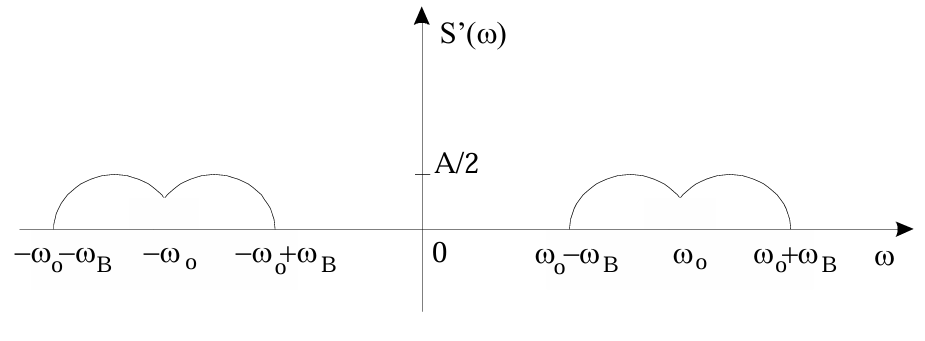
\includegraphics[scale = 0.6]{Esempio di segnale trasformato in Fourier.PNG}
\end{figure}

Si può campionare ad una frequenza minore della condizione di Nyquist grazie ai buchi nelle bande di frequenza. \newline 

\newpage 

\section{Codifica PCM e sua applicazione a segnali di interesse pratico} 

Lo schema a blocchi di un sistema che utilizza la modulazione impulsiva codificata (PCM: Pulse Code Modulation): 

\begin{figure}[h]
    \centering
    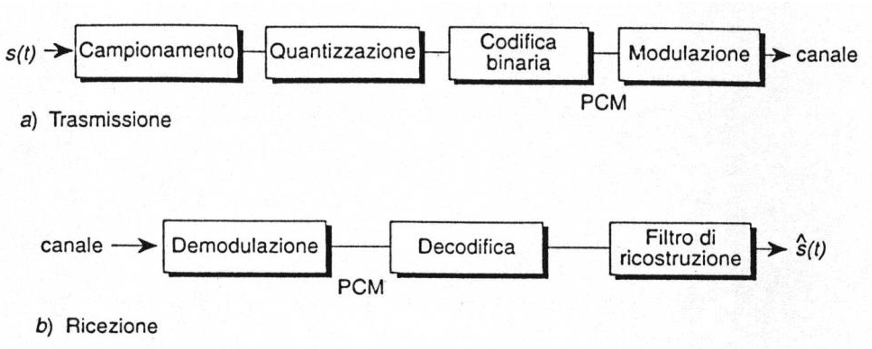
\includegraphics[scale = 0.6]{PCM Schema a blocchi.PNG}
\end{figure}

Il punto di partenza è costituito da un segnale analogico s(t) di banda limitata, 
che viene campionato, in accordo con il teorema di campionamento,con una frequenza almeno pari a 2B. \newline 

In tal modo, il segnale variabile in modo continuo nel tempo viene trasformato in una seguenza, discreta, di campioni. \newline 

Le ampiezze dei campioni, peraltro, possono essere qualisiasi (compatibilmente con la dinamica del segnale s(t)). \newline 

Per ricavare la frequenza di cifra del segnale PCM, è sufficiente guardare alle operazioni che conducono dal segnale analogico s(t) al segnale numerico PCM: 

\begin{itemize}
    \item il campionamento comporta che venga prelevato un campione ogni $T_o = \frac{1}{f_o} \leq \frac{1}{2B} [s]$ (la frequenza di campionamento è stata qui indicata con $f_o$)
    \item il tenpo riservato alla trasmissione di un simbolo M-ario non può eccedere $\frac{1}{2B}$: si assume, di solito, il valore massimo 
    \item sostituendo una sequenza binaria al generico simbolo M-ario, ciascuna cifra binaria avrà durata massima pari a $\frac{1}{2B \cdot \log_2 M}$ in quanto il tempo riservato alla trasmissione di un simbolo M-ario deve ora essere ripartito tra i $\log_2 M$ simboli binari
\end{itemize}


La frequenza di cifra del PCM sarà: 

{
    \Large 
    \begin{equation}
        F_c = 2B \cdot \log_2 M
    \end{equation}
}

Per i segnali di interesse pratico, i valori di B e di M sono stardatizzati. \newline 

\newpage 
.
\newpage
.
\newpage
 
\chapter{Trasformata di Hilbert} 

\begin{figure}[h]
    \centering
    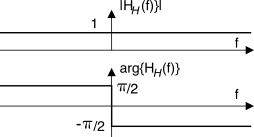
\includegraphics[scale = 2]{Filtro di Hilbert.png}
\end{figure}  

\newpage 

\section{Cosa è la trasformata di Hilbert} 

La trasformata di Hilbert è una particolare rappresentazione, che, contrariamente ad altre trasformate 
non realizza un cambiamento del dominio di definizione. \newline 

In altre parole, a partire da una funzione del tempo s(t), la trasformata di Hilbert $s^{\sim} (t)$ è ancora una funzione del tempo. \newline 

$s^{\sim} (t)$ si ottiene come uscita da un filtro, detto filtro di Hilbert, caratterizzato dalla funzione di trasferimento: 

{
    \Large 
    \begin{equation}
        H_H (f) = 
        \begin{cases}
            -\jmath \text{ per } f>0  \\ 
            0 \text{ per } f = 0 \\ 
            \jmath \text{ per } f<0
        \end{cases}
    \end{equation}
}

in termini di parte reale e parte immaginaria, avremo: 

{
    \Large 
    \begin{equation}
        \abs{H_H (f)} = 
        \begin{cases}
            1 \text{ per } f \neq 0 \\ 
            0 \text{ per } f = 0
        \end{cases}
    \end{equation}
}

{
    \Large 
    \begin{equation}
        \arg{H_H (f)} = 
        \begin{cases}
            -\frac{\pi}{2} \text{ per } f > 0 \\ 
            0 \text{ per } f = 0 \\ 
            \frac{\pi}{2} \text{ per } f < 0
        \end{cases}
    \end{equation}
}

in termini di parte reale e fase. \newline 

Schematizzando i filtri ed i segnali, avremo che: 

\begin{figure}[h]
    \centering
    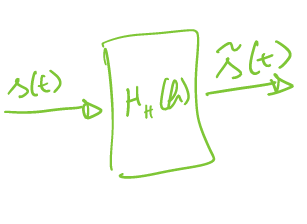
\includegraphics[scale = 0.5]{trasformata di Hilbert segnali con filtro.PNG}
\end{figure} 

Nel dominio della frequenza, si ha: 

{
    \Large 
    \begin{equation}
        S^{\sim} (f) = H_H (f)S(f)
    \end{equation}
}

dove $S(f)$ è la trasformata di Fourier di s(t) mentre $S^{\sim}(f)$ è la trasformata di Fourier di $s^{\sim} (t)$. \newline 

Sapendo la relazione tra frequenza e tempo, possiamo sapere che la risposta impulsiva del filtro di Hilbert nel tempo è: 

{
    \Large 
    \begin{equation}
        h_H (t) = \frac{1}{\pi t}
    \end{equation}
}

Grazie alle proprietà della trasformata di Fouerier, sapendo che $H_H (f)$ è una funzione puramente immaginaria e dispari, 
anche $h_H (t)$ è puramente reale e dispari. \newline 

L'operazione di trasformazione inversa di Hilbert, che consente di riottenere il segnale s(t) a partire da $s^{\sim} (t)$ richiede, in realtà, una nuova trasformata di Hilbert:

{
    \Large 
    \begin{equation}
        \begin{split}
            S^{\approx} 
            &= 
            H_H(f) S^{\sim} (f) 
            \\ 
            &= 
            H_H(f) H_H(f) S(f) 
            \\ 
            &= 
            -S(f)
        \end{split}
    \end{equation}
}

Questa relazione vale per tutti i valori $f \neq 0$. \newline 

In $f=0$, il valore $S(0)$, se diverso da zero, viene annullato, e non potrà essere più recuperato. \newline 

In particolare, se il segnale ha valore medio diverso da zero, questo si tradurrebbe nella presenzza nello spettro di una delta di Dirac posizionata nell'origine. \newline 

Di conseguenza, possiamo concludere che la classe dei segnali per cui è applicabile la trasformata di Hilbert è quella dei segnali a valor medio nullo. \newline 

Dal punto di vista ingegneristico: 

\begin{figure}[h]
    \centering
    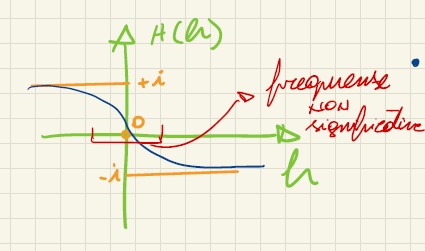
\includegraphics[scale = 0.5]{Considerazioni filtro di Hilbert in frequenza.PNG}
\end{figure}  

inoltre, è difficilmente realizzabile un filtro con una transizione così brusca, quindi, 
generalmente, la transizione è "smussata". \newline 

\newpage 
\chapter{DFT} 

\begin{figure}[h]
    \centering
    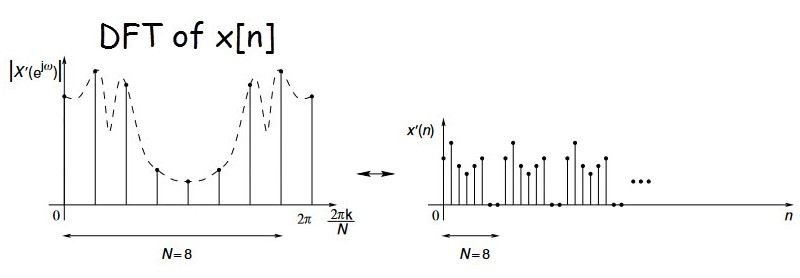
\includegraphics[scale = 0.7]{DFT.jpg}
\end{figure}  

\newpage 

\section{Introduzione alla trasformata discreta di Fuorier (DFT)}

La trasformata discreta di Fourier, comunemente nota in letteratura con l'acronimo DFT (Discrete Fourier Transform) 
risponde all'esigenza di implementare al calcolatore la trasformata di Fourier di una funzione del tempo. \newline 

Si considerino la funzione h(t) e la sua trasformata di Fourier H(f) in figura: 

\begin{figure}[h]
    \centering
    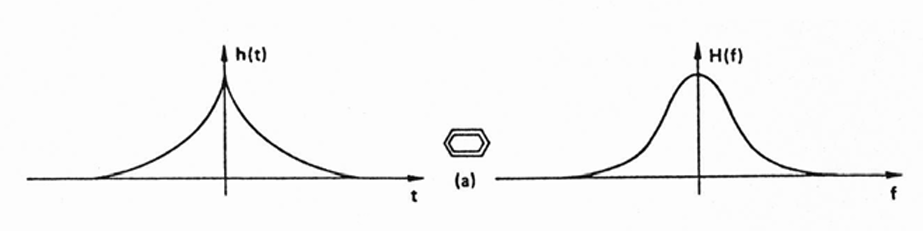
\includegraphics[scale = 0.7]{h(t) e H(f).PNG}
\end{figure} 

Per determinare la trasformata di Fourier di h(t) mediante tecniche di analisi digitale, 
è necessario campionare la funzione h(t). \newline 

Il campionamento è relaizzato moltiplicando h(t) per la sequenza campionante $\Delta_o (t)$. \newline 

Quindi, sapendo che $\Delta_o (t)$ è la seguente: 

\begin{figure}[h]
    \centering
    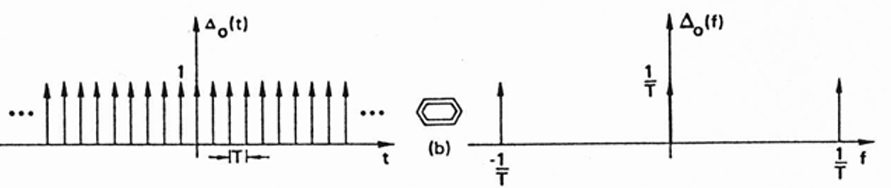
\includegraphics[scale = 0.7]{Treno di impulsi Delta_o (t).PNG}
\end{figure} 

$h(t) \cdot \Delta_o (t)$ sarà: 


\begin{figure}[h]
    \centering
    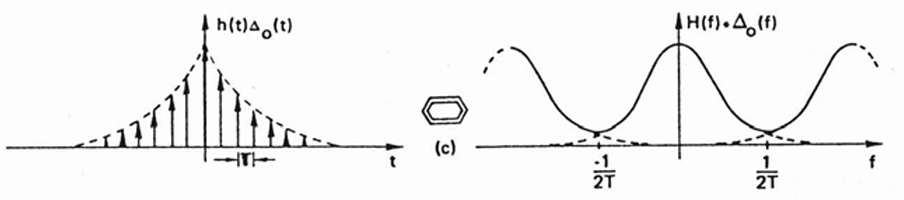
\includegraphics[scale = 0.7]{h(t) moltiplicata per il treno di impulsi.PNG}
\end{figure} 

Analizzando la figura, notiamo che la sequenza è costituita da una sequenza di implusi matematici (Delta di Dirac) 
distanziati di T l'uno dall'altro. \newline 

Il risultato del campionamento è, in Fourier, il segnale originale replicato infinte volte, centrato su un multiplo della frequenza di campionamento $\frac{1}{T}$. \newline 

Se la frequenza non è sufficientemente grande, compare il fenomeno dell'aliasing, per cui tali repliche risultano sovrapposte. \newline 

Procedendo coi passaggi, avremo che: 

\begin{figure}[h]
    \centering
    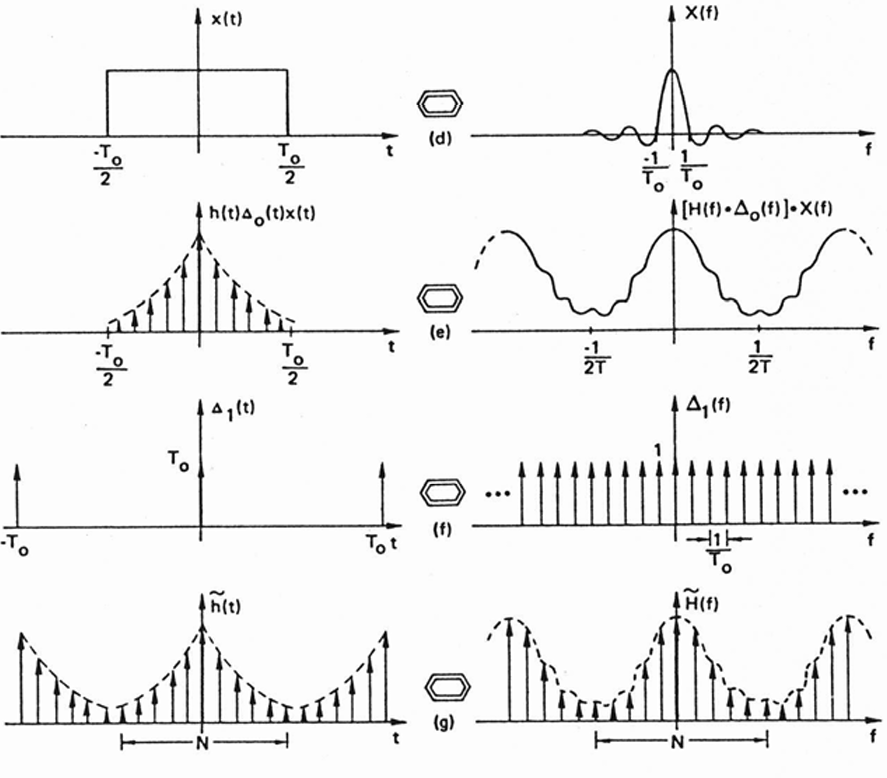
\includegraphics[scale = 0.7]{Altri passaggi per la DFT.PNG}
\end{figure} 

\newpage 

Come notiamo dalla figura, il campionamento nel dominio del tempo ha prodotto una funzione periodica in frequenza, 
mentre il campionamento nel dominio della frequenza ha prodotto una funzione periodica nel tempo. \newline 

Ciascun periodo, nel tempo e in frequenza, contiene N campioni. \newline 

\newpage 

Invece, analizzando un altro esempio di segnale, l'esponenziale bilaterale unilatera, e che quindi si sviluppa solo in $t \geq 0$ 
e ponendo la finestra di campionamento non centrata nell'origine, notiamo che: 

\begin{figure}[h]
    \centering
    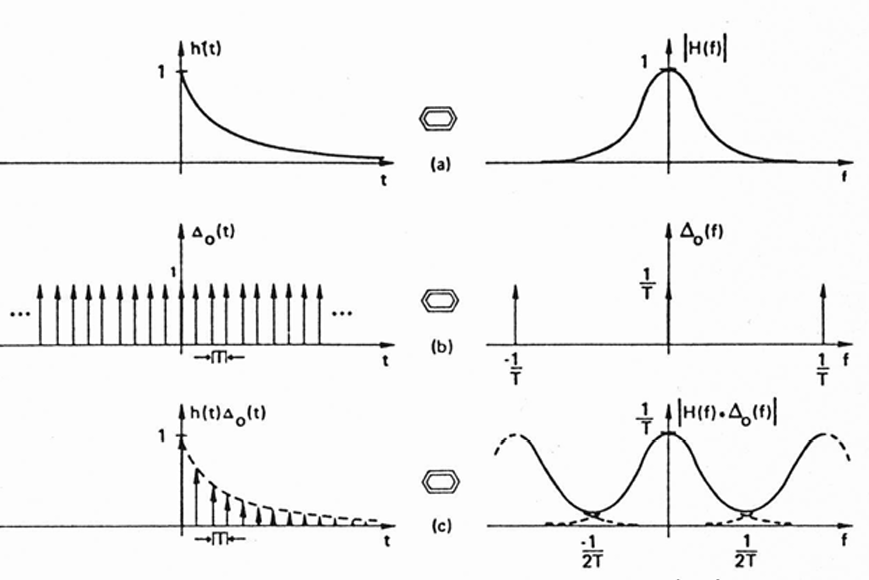
\includegraphics[scale = 0.7]{Campionamento segnale espnenzianziale unilatera.PNG}
\end{figure} 

\newpage

Formalizzando le figure in formule matematiche, notiamo che: 

{
    \Large 
    \begin{equation}
        \begin{split}
            h(t) \Delta_o (t) 
            &= 
            h(t) 
            \sum_{k = - \infty}^{\infty} 
            \delta (t - kT) 
            \\ 
            &= 
            \sum_{k = - \infty}^{\infty}
            h(kT) 
            \delta (t - kT)
        \end{split}
    \end{equation}
}

Assumendo N campioni, signfica moltiplicare la funzione precedente per x(t). \newline 

Utilizzando le figure: 

\begin{figure}[h]
    \centering
    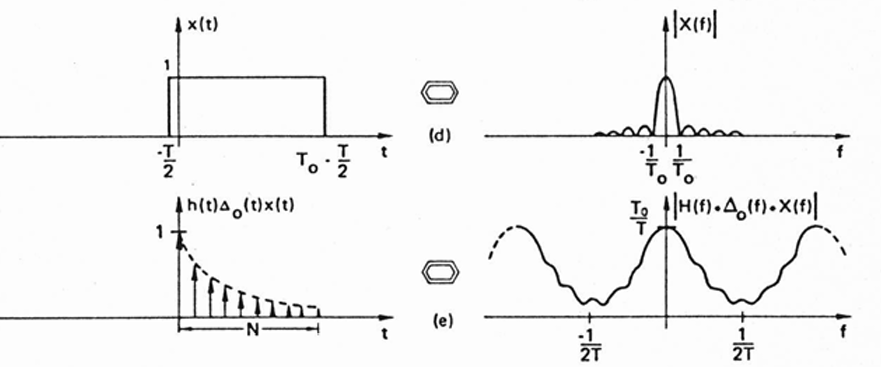
\includegraphics[scale = 0.7]{Campionamento segnale espnenzianziale unilatera step 2.PNG}
\end{figure} 

Formalizzando: 

{
    \Large 
    \begin{equation}
        \begin{split}
            h(t) \Delta_o (t) x(t) 
            &= 
            [ h(t) \sum_{k = -\infty}^{\infty} \delta (t - kT) ] x(t) 
            \\ 
            &= 
            \sum_{k = 0}^{N-1} 
            h(kT) \delta (t - kT)   
        \end{split}
    \end{equation}
}

Alla funzione campionante nel domnio della frequenza, $\Delta_l (f)$, corrispondente nel dominio del tempo: 

\begin{figure}[h]
    \centering
    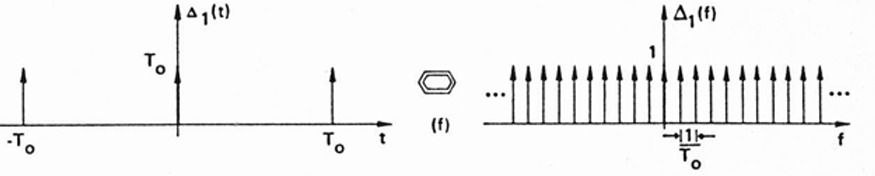
\includegraphics[scale = 0.7]{Delta_l (f).PNG}
\end{figure} 

{
    \Large 
    \begin{equation}
        \Delta_l (t) = T_o \sum_{r = -\infty}^{\infty} \delta (t - rT_o)
    \end{equation}
}

Facendo la convoluzione, notiamo che: 

\begin{figure}[h]
    \centering
    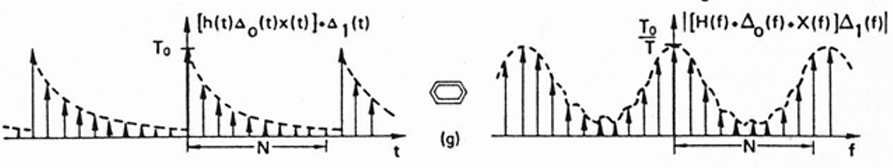
\includegraphics[scale = 0.7]{Convoluzione esponenziale DFT.PNG}
\end{figure} 

{
    \Large 
    \begin{equation}
        \begin{split}
            h^{\sim} (t) 
            &= 
            [h (t) \Delta_o (t) x(t)] * \Delta_l (t) 
            \\ 
            &= 
            [\sum_{k = 0}^{N-1} h(kT) \delta(t - kT)] 
            * 
            [T_o \sum_{r = -\infty}^{\infty} \delta (t-rT_o)]
            \\ 
            &= 
            T_o \sum_{r = \infty}^{\infty} [\sum_{k = 0}^{N-1} h(kT) \delta (t - kT -rT_o)]    
        \end{split}
    \end{equation}
}

\newpage 

\section{Casi di pratico interesse interesse}

Rispetto all'aspetto analitico, si prediligerà l'aspetto grafico nel tema della DFT. \newline 

\newpage

\subsection{Forme d'onda periodiche a banda limitata: finestra di campionamento uguale al periodo}

\begin{figure}[h]
    \centering
    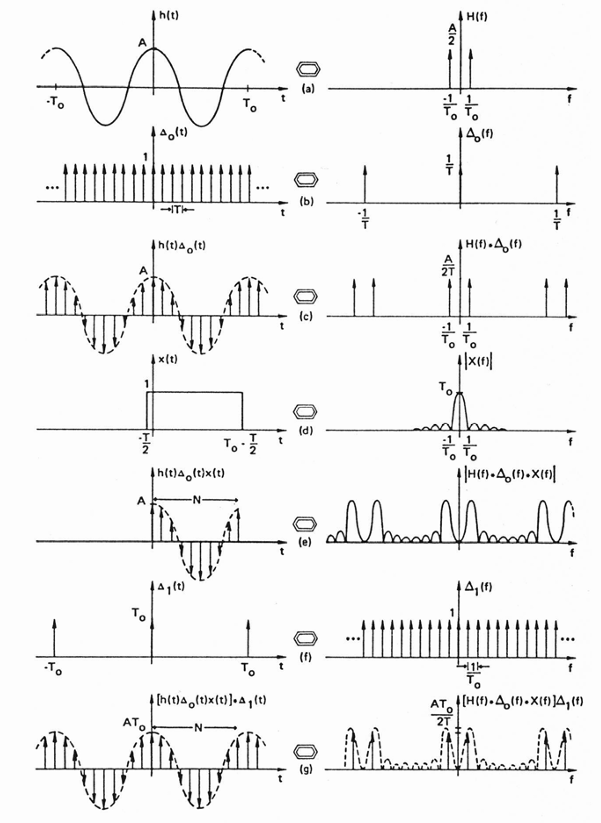
\includegraphics[scale = 0.8]{Forma d'onda periodica a banda limitata finestra di campionamento uguale al periodo.PNG}
\end{figure} 

Scorrendo rapidamente le varie parti per produrre la DFT, notiamo che: 

\begin{itemize}
    \item il campionamento nel dominio del tempo non produce aliasing 
    \item il campionamento nel dominio del tempo produce una scalatura delle ampiezze nel dominio delle frequenze, per cui l'area originale (A/2) della Delta di Dirac viene ridotta di un fattore 1/T, quindi diventa A/2T 
    \item la finestra di campionamento include esattamente un periodo della funzione cosinusoidale, e gli N campioni nel dominio del tempo sono contenuti entro questo periodo 
    \item il risultato del prodotto nel dominio del tempo fra la forma d'onda campionata e la finestra di campionamento ha uno spettro fortemente distorto rispetto alla H(f) originale 
    \item quando, però, si effettua il campionamento nel dominio della frequenza, questa distorsione sparisce
\end{itemize}

\newpage 

\subsection{Forme d'onda periodiche a banda limitata: finestra di campionamento diversa dal periodo}
\include{10 - Unità logaritmiche} 
\chapter{Interferenza di intersimbolo} 

\begin{figure}[h]
    \centering
    \includegraphics[scale = 1]{DigitalModulation_clip_image114.jpg}
\end{figure}  

\newpage 

\section{Da impulsi rettangolari alle forme d'onda reali}

Nell'accezione comune, le forme d'onda utilizzate in una trasmissione numerica hanno durata finita; 
in particolare, è frequente il caso in cui si utilizzino impulsi rettangolari di durata uguale o minore di un intervallo caratteristico, denominato tempo di simbolo. \newline 

\begin{figure}[h]
    \centering
    \includegraphics[scale = 0.8]{Impulsi rettangolari.PNG}
\end{figure}  

La trasmissione di un segnale numerico con queste caratteristice avrebbe, a rigore, bisogno di una banda infinita perchè ha fronti 
d'onda a pendenza elevata, nel caso di impulsi rettangolari la transizione è immediata, quindi banda illimitata. \newline 

Quando un segnale numerico si trova a transitare attraverso un filtro, ad esempio un canale di trasmissione, esso verrà inevitabilmente distorto. \newline 

Il segnale rettangolare visto in precedenza, dopo il passaggio ad un filtro, si può presentare come segue: 

\begin{figure}[h]
    \centering
    \includegraphics[scale = 0.8]{Impulsi rettangolari dopo un filtro.PNG}
\end{figure} 

Confrontando lo stesso segnale, prima e dopo il filtro, notiamo che gli impulsi binari, che sono ben distinti nel segnale di ingresso $s_i (t)$ rislutano sovrapposti nel segnale di uscita $s_u (t)$. \newline 

Trattandosi di un fenomeno (indesiderato) di interazione tra simboli, si è soliti parlare di inteferenza intersimbolica (in inglese ISI: InterSymbol Interference). \newline 

I simboli interferenti possono riferirsi allo stesso (e unico) segnale, o, nel caso delle comunicazioni, il mezzo trasmissivo è condiviso tra più utenti a divisione di tempo, 
in cui si usa lo stesso mezzo trasmissivo tra sorgente-destinazioni: in questo casa ci saranno degli effetti di mutuo disturbo tra le diverse comunicazioni. \newline 

\newpage 

\section{Diagramma ad occhio} 

Uno strumento molto utile nel capire l'effetto dell'ISI in un segnale è quello del diagramma ad occhio. \newline 

Un esempio di diagramma ad occhio: 

\begin{figure}[h]
    \centering
    \includegraphics[scale = 0.8]{Esempio di diagramma ad occhio.PNG}
\end{figure} 

Dal punto di vista concettuale, il diagramma ad occhio si ottiene generando tutte le possibili sequenze di simboli binari e graficandone sovrapposti gli andamenti a valle del canale distorcente. \newline 

Un esempio di diagramma ad occhio step-by-step: 

\begin{figure}[h]
    \centering
    \includegraphics[scale = 0.8]{Diagramma ad occhio step-by-step.PNG}
\end{figure} 

Confrontando diversi diagrammi ad occhio di diverse trasmissioni, possiamo avere i seguenti casi: 

\begin{figure}[h]
    \centering
    \includegraphics[scale = 0.8]{Diversi diagrammi ad occhio.PNG}
\end{figure} 

\newpage 

L'apertura dell'occhio dà la massima distanza tra i due livelli di decisione. \newline 

Quindi, i casi (c) e (d) sono migliori rispetto ai casi (a) e (b). \newline 

Diagramma ad occhio ideali possono essere ottenuti con una scelta adeguata della funzione di trasferimento del canale, ovvero introducendo una opportuna equalizzazione della funzione di trasferimento di un canale preassegnato. \newline 

\newpage 

\section{Sintesi di un filtro per annullare l'ISI} 

Idealmente, è possibile annullare l'ISI; nella realtà, si cercherà di diminuirlo di tanto. \newline 
Inoltre, l'annullamento non è sempre conseguibile.\newline 

In particolare se la banda B del canale è minore della metà della frequenza di simbolo del segnale numerico, 
in formule: 

{
    \Large 
    \begin{equation}
        B < \frac{F_s}{2} = \frac{1}{2 T_s}    
    \end{equation}
} 

l'obbiettivo dell'annullamento dell'interferenza di intersimbolo non potrà essere, in alcun modo, conseguito. \newline 

Per una data frequenza di simbolo, caratteristica della trasmissione, esiste una larghezzza di banda minima per la banda del canale, al di sotto della quale l'ISI non può essere compensata. \newline 

Dualmente, un sistema caratterizzato da una banda B, se necessario opportunamente equalizzato, può annullare l'interferenza intersimbolica di sistemi con frequenza di simbolo al più uguale a 2B, ma non maggiore. \newline 

Ad esempio, se $B = 1 MHz$, non si può annullare l'ISI di un sistema con frequenza di simbolo $F_s > 2 Mbit/s$. \newline 

Quindi, ponendo $B \geq \frac{F_s}{2}$, possiamo ora fornire alcuni esempi di funzioni di trasferimento in grado di annullare l'interferenza intersimbolica. \newline 

La funzione $H(\omega)$, rappresenta la funzione di traferimento della cascata di reti 2-porte: 

\begin{figure}[h]
    \centering
    \includegraphics[scale = 0.8]{Cascata reti 2-porte.PNG}
\end{figure} 

Analizzando la cascata di 2-porte, abbiamo che: 
\begin{itemize}
    \item la rete di formazione degli impulsi $R(\omega)$ 
    \item la funzione di trasferimento del mezzo trasmissivo $L(\omega)$ 
    \item la funzione equalizzatrice in ricezione $E(\omega)$
\end{itemize}

Quindi: 

{
    \Large 
    \begin{equation}
        H(\omega) = R(\omega)L(\omega)E(\omega)
    \end{equation}
}

La rete di formazione degli impulsi, in particolare, trasforma una sequenza di Delta di Dirac in ingresso (cui è associata, in senso stretto, l'informazione) 
in una sequenza di impulsi di durata finita: 

\begin{figure}[h]
    \centering
    \includegraphics[scale = 0.8]{Rete forazione degli impulsi.PNG}
\end{figure} 

\newpage 

L'informazione trasmessa è chiaramente già contenuta nella successione di Delta di Dirac, ma tale successione non è un segnale fisico (in quanto un impulso matematico ideale non può essere ottenuto in pratica), 
mentre tale risulta la successione di impulsi rettangolari. \newline 

Una prima importante classe di funzioni in grado di annullare l'interferenza di intersimbolo è quella che va sotto il nome di "funzione di trasferimento a coseno rialzato". \newline 

L'espressione analitica di $H(\omega)$ per questa classe di funzioni è la seguente: 

{
    \Large 
    \begin{equation}
        H(\omega) 
        = 
        \begin{cases}
            H_o \text{ per } \abs{\omega} \leq \pi \frac{1 - b}{T_s} \\ 
            \frac{H_o}{2}[1 - \sin(\frac{\abs{\omega} T_s - \pi}{2b})] \text{ per } \pi \frac{1 - b}{T_s} \leq \abs{\omega} \leq \pi \frac{1 + b}{T_s} \\ 
            0 \text{ per } \abs{\omega} \geq \pi \frac{1 - b}{T_s}
        \end{cases}
    \end{equation}
}

dove $H_o$ è una costate reale, mentre b è detto "fattore di roll-off" e varia tra 0 e 1. \newline 

Dal punto di vista grafico e al variare di b, $H(\omega)$ sarà: 

\begin{figure}[h]
    \centering
    \includegraphics[scale = 0.8]{Funzione di trasferimento a coseno rialzato.PNG}
\end{figure}

La largehezza di banda, espressa in Hz, della funzione di trasferimento a coseno rialzato, vale: 

{
    \Large 
    \begin{equation}
        \begin{split}
            B 
            &= 
            \frac{1}{2 \pi}
            (\pi \frac{1 + b}{T_s}) 
            \\
            &= 
            \frac{1 + b}{2 T_s}
        \end{split}
    \end{equation}
}

Il valore minimo di B è quando $b=0$, che, appunto, è pari a $\frac{1}{2T_s}$. \newline 

Ciò conferma le precedenti considerazioni sulla banda minima in grado di annullare l'ISI e, dall'altra, 
evidenzia che, se l'obbiettivo è quello di minimizzare l'occupazione spettrale, la scelta $b=0$ è la più conveniente. \newline 

Ma, $H(\omega)$ con $b=0$ è impossibile da realizzare con componenti fisici reali (si tratterebbe di un filtro passa-basso ideale), 
mentre la funzione con $b=1$ presenta una transizione più graduale, quindi sarà realizzabile in modo relativamente semplice ed efficiente. \newline 

Inoltre il valore b ottimo dipende non solo da quello che accade nel dominio di $\omega$, 
bensì anche quello che succede nel dominio del tempo. \newline 

Anti-trasformando $H(\omega)$, avremo: 

{
    \Large 
    \begin{equation}
    h(t) 
    = 
    H_o 
    \frac{1}{T_s} 
    \frac{\sin(\frac{\pi}{T_s} t)}{\frac{\pi}{T_s} t}
    \frac{\cos(\frac{\pi}{T_s}) bt}{1 - \frac{4}{T_s ^{2} }b^{2} t^{2}}         
    \end{equation}
}

\begin{figure}[h]
    \centering
    \includegraphics[scale = 0.8]{Anti-trasformata della funzione coseno rialzato.PNG}
\end{figure}

h(t) ha il significato di risposta impulsiva. \newline 

Dalla figura, notiamo che: 

{
    \Large 
    \begin{equation}
        \begin{cases}
            h(0) = h_o \\ 
            h(k T_s) = 0 \text{ per } k = \pm 1, \pm 2, ...
        \end{cases}
    \end{equation}
}

Da queste equazioni, notiamo che, in $t=0$ si annulla l'ISI, e negli altri istanti k non distorce la funzione di ingressi. \newline 

Inoltre, osservando la figura, notiamo che, all'aumentare di b, le code della h(t) risultano maggiormente confinate introrno all'asse dei tempi. \newline 

Quindi, tipicamente, si sceglie un b compreso tra 0.6 e 0.8. \newline 

Inoltre, possiamo notare che la famiglia delle funzioni a coseno rialzato verifica la seguente proprietà: 

{
    \Large 
    \begin{equation}
        \begin{split}
            H_o (\omega_o) 
            &= 
            \sum_{n = -\infty}^{\infty}
            H (\omega_o + n \frac{2 \pi}{T_s})
            \\ 
            &= 
            T_s h_o 
            \text{ per }
            -\frac{\pi}{T_s} \leq \omega_o \leq \frac{\pi}{T_s} 
        \end{split}
    \end{equation}
}

In altre parole, considerata una generica pulsazione $\omega_o$ nell'intervallo $[- \frac{\pi}{T_s}, \frac{\pi}{T_s}]$
la funzione $H_o (\omega_o)$ che si ottiene sommando i valori assunti dalla $H(\omega)$ in $\omega_o$ ed in punti che distano da $\omega_o$ per multipli interi 
di $\frac{2 \pi}{T_s}$ è costante.\newline 

Questa proprietà è nota come criterio di Nyquist, è di validità generale e consente di definire una famiglia di funzioni, 
appunto note come funzioni della classe di Nyquist, tutte in grado di annullare l'interferenza intersimbolica. \newline 

Ritornando a $H(\omega)$, $E(\omega)$ è la rete equilizzatrice in ricezione. \newline 

Una volta scelto il mezzo trasmissivo $L(\omega)$ è assegnata; ad esempio, nel caso di un cavo coassiale, sotto l'ipotesi di piccole perdite, si può scrivere: 

{
    \Large 
    \begin{equation}
        L(\omega) = \exp [- \sqrt{\frac{\omega}{\omega_o}} (1+ \jmath) -\jmath \omega t_c]
    \end{equation}
}

dove $\omega_o$ è una pulsazione caratteristica, mentre $t_c$ è il tempo di propagazione delle onde elettromagnetiche nel mezzo. \newline 

Il prodotto $R(\omega) \cdot L (\omega)$ appartiene alla classe di Nyquist; 
in generale, è quindi necessario introdurre l'opportuna correzione attraverso $E(\omega)$. \newline 

Graficamente: 

\begin{figure}[h]
    \centering
    \includegraphics[scale = 0.8]{Spettro della cascata delle reti 2-porte.PNG}
\end{figure}


Chiaramente deve essere: 

{
    \Large 
    \begin{equation}
        E(\omega) R(\omega) = \frac{H(\omega)}{L(\omega)}
    \end{equation}
}

Una soluzione molto frequente è quella di porre: 

{
    \Large 
    \begin{equation}
        \abs{E(\omega)} = \abs{R(\omega)} = \sqrt{\frac{\abs{H(\omega)}}{\abs{L(\omega)}}}
    \end{equation}
}

Scegliendo arbitrariamente la fase di $E(\omega)$. \newline 

Se il rapporto $\frac{H(\omega)}{L(\omega)}$ è reale, si può porre semplicemente: 

{
    \Large 
    \begin{equation}
        E(\omega) = R^{*} (\omega)
    \end{equation}
}

\newpage 
. 
\newpage 
. 
\newpage
\include{12 - Richiami di teoria della probabilità}
\chapter{Processi stocastici}

\begin{figure}[h]
    \centering
    \includegraphics[scale = 1.5]{Processo stocastico.png}
\end{figure}   

\newpage 

\section{Processi stocastici: cosa sono}

I segnali aleatori vengono comunemente denominati processi stocastici. \newline 

Per un processo stocastico non è definibile, e dunque calcolabile, la trasformata di Fourier perchè 
la trasformata di Forurier presuppone la conoscenza dell'andamento del segnale. \newline 

L'evoluzione di un processo stocastico può essere descritto solo statisticamente. \newline 

Piuttosto che usare come dominio la frequenza e la trasformata di Forurier, 
per un processo stocastico si sceglierà di utilizzare lo spettro di potenza del processo. \newline 

Consideriamo la seguente figura: 

\begin{figure}[h]
    \centering
    \includegraphics[scale = 1]{Processo stocastico segnali.PNG}
\end{figure}  

Tutti questi andamenti sono di un processo stocastico x(t). \newline 

Al fine di descrivere statisticamente il processo, si può fissare l'attenzione sul valore assunto da x(t) in un generico istante (ad esempio $t_1$) 
e valutare la densità di probabilità $f_1 (x_1; t_1)$ della variabile aleatoria estratta $x_1 = x(t_1)$. \newline 

Allo steso modo si può considerare un altro istante $t_2$ e valutare la corrispondente $f_2 (x_2; t_2)$, 
che in questo caso rappresenterà la densità di probabilità della variabile aleatoria estratta $x_2 = x(t_2)$. \newline 

La procedura può essere estesa ad un numero arbitrario di istanti (e quindi di variabili aleatorie estratte). \newline 

Una descrizione più accurata si ottiene prendendo in esame, contemporaneamente, due istanti generici (ad esempio $t_1$ e $t_2$) e valutando la densità di probabilità congiunta $f_{12} (x_1, x_2; t_1, t_2)$. \newline 

La probabilità congiunta $f_{12} (x_1, x_2; t_1, t_2)$ molte delle volte è una soluzione alla maggior parte dei problemi. \newline 


\newpage 

\section{Medie di insieme} 

Per le variabili aleatorie estratte dal processo sono calcolabili le medie di insieme. \newline 

Consideriamo il valore medio in $x_1$, che sarà dato da: 

{
    \Large 
    \begin{equation}
        <x_1> 
        = 
        \int_{- \infty}^{+\infty}
        x_1 f_1 (x_1; t_1) dx_1
    \end{equation}
}

Il momento congiunto di ordine (1, 1) delle variabili $x_1$ e $x_2$ si otterrà come: 

{
    \Large 
    \begin{equation}
        <x_1 x_2> 
        = 
        \int_{- \infty}^{+\infty}
        \int_{- \infty}^{+\infty}
        x_1 x_2 f_{12} (x_1, x_2; t_1, t_2) 
        dx_1
        dx_2
    \end{equation}
}

Il momento congiunto di ordine (1, 1), che rappresenta la correlazione tra le variabili aleatorie estratte $x_1$ e $x_2$; 
prende il nome di autocorrelazione statistica del processo e si indica con $R(t_1, t_2)$. \newline 

Si noti che nelle densità di probabilità, in $<x_1>$ e $<x_1 x_2>$ le variabili aleatorie sono le $x_i$ mentre il tempo svolge il ruolo di paramentro. \newline 

In generale, le densità di primo ordine sono diverse al variare dell'istante $t_i$ considerato e le densità di ordine superiore 
dipendono singolarmente dagli istanti $t_i, t_j, ..., t_k$. \newline 

Più frequentemente, si può ritenere vera la circostanza che una traslazione arbitraria dall'origine dei tempi dell'intero 
processo non ne modifichi le caratteristiche statistiche. \newline 


\newpage 
\section{Stazionarietà e ergodicità}
Con riferimento alle definizioni precedenti, ciò comporta che: 

\begin{itemize}
    \item la densità del primo ordine è indipendete da t, ed è quindi la stessa per ogni possibile variabile aleatoria estratta 
    \item la densità del secondo ordine dipende solo dalla differenza $\tau = t_2 - t_1$
    \item la densità di probabilità di ordine n dipende solo dagli $n-1$ parametri
\end{itemize}

Un processo di questo tipo si dice stazionario in senso stretto e, per esso, la densità di probabilità del 
primo e del secondo ordine si scrivono $f(x)$ e $f_{12} (x_1, x_2; \tau)$ rispettivamente. \newline 

Accanto alla stazionarietà in senso stretto, si può definire anche la stazionarietà in senso lato. \newline 

Si può defnire un processo con stazionarietà in senso lato se ha valore medio $<x_1>$ è indipendente da t e la cui 
autocorrelazione statistica $<x_1 x_2>$ dipende solo dalla differenza $\tau = t_2 - t_1$. \newline 

La stazionarietà in senso stretto implica, ovviamente, la stazionarietà, mentre non è vero il viceversa. \newline 

La proprietà di stazionarietà è propedeutica ad un altro fondamentale concetto: quello di ergodicità. \newline 

In un processo ergodico ogni realizzazione è tipica del processo, nel senso che la sua osservazione per un tempo sufficientemente lungo consente di estrarre tutte le 
proprietà del processo stesso. \newline 

L'accuratezza della stima può essere arbitrariamente migliorata aumentando il livello di risoluzione orizzontale (vale a dire, riducendo l'estensione degli intervalli) 
ed assumendo un valore di N via via più elevato. \newline 

In figura un esempio di intervalli sempre più stretti: 

\begin{figure}[h]
    \centering
    \includegraphics[scale = 0.7]{Intervalli più stretti.PNG}
\end{figure}  


L'istogramma può essere utilizzato per stimare la densità di probabilità del secondo ordine o una qualunque media di insieme. \newline 

Un processo ergodico, in tutte le sue densità di probabilità di qualasiasi ordine, si dirà 
generalmente, ergodico. \newline 

Se le considerazioni qualitative precedenti fossero formalizzate in termini rigorosamente analitici, 
ci saremo resi conto che l'ergodicità presuppone la stazionarietà. \newline 

In altri termini, non può essere ergodico un processo che non è stazionario. \newline 

La maggior parte dei processi reali non sono intriscamente ergodici, ma, possono essere separati e/o ridotti in processi 
più semplici e singolarmente ergodici.\newline 


Per un processo stocastico, possiamo considerare anche le medie temporali. \newline 

Il valore medio temporale di una generica realizzazione del processo x(t) è definito come: 

{
    \Large 
    \begin{equation}
        \overline{x(t)} 
        =
        \lim_{\Delta t \to \infty}
        \frac{1}{\Delta t}
        \int_{-\frac{\Delta t}{2}}^{\frac{\Delta t}{2}} 
        x(t) dt  
    \end{equation}
}

$\overline{x(t)} = <x> $ in parole, possiamo vedere il valore medio temporale come il valore medio statistico. \newline 

Invece, l'autocorrelazione temporale possiamo definirla come: 

{
    \Large 
    \begin{equation}
        \overline{R (\tau)} 
        = 
        \lim_{\Delta t \to \infty}
        \frac{1}{\Delta t}
        \int_{-\frac{\Delta t}{2}}^{\frac{\Delta t}{2}} 
        x(t) 
        x(t + \tau)
        dt  
    \end{equation}
}

in cui $\tau = t_2 - t_1$ e $\overline{x(t)} = <x_1 x_2> $.  \newline 


La generica realizzazione del processo, una volta specificata (vale a dire, misurata o registrata), 
può essere riguardata come un particolare segnale determinato a potenza finita. \newline 

Per esso si può definire una densità spettrale (o semplicemente spettro di potenza) $p(\omega)$ che, 
in accordo con i segnali determinati, sarà data da: 

{
    \Large 
    \begin{equation}
        p(\omega) = \lim_{\Delta t \to \infty} \frac{\abs{X_\Delta (\omega)}^{2}}{\Delta t}
    \end{equation}
}


dove $X_\Delta (\omega)$ è la trasformata di Foruier del segnale che si ottiene considerando x(t) entro un intervallo, 
centrato nell'origine e di estensione $\Delta t$. \newline 

\newpage 

\section{Processo ergodico e il teorema di Wiener-Khintchine}

Nel caso di un processo erogodico, le medie di insieme (vale a dire le medie statistiche) coincidono con le medie temporali e possono essere 
calcolate a partire da un'unica e generica realizzazione del processo. \newline 

Per questo tipo di processi, possiamo enunciare il seguente teorema, il teorema di Wiener-Khintchie: 
se il processo x(t) è stazionario ed ergodico, almeno nella sua autocorrelazione, lo spettro di potenza del processo ad esso associato risulta 
la trasformata di Fourier della sua autocorrelazione statistica $R(\tau)$. \newline 


Sempre in virtù dell'ergodicità e delle proprietà ad esse associate, si può osservare che:

{
    \Large 
    \begin{equation}
        \begin{split}
            P 
            &= 
            \lim_{\Delta t \to \infty}
            \frac{1}{\Delta t}
            \int_{-\frac{\Delta t}{2}}^{\frac{\Delta t}{2}}
            x^{2} (t) dt 
            \\ 
            &= 
            \overline{R (0)}
            \\ 
            &= 
            R(0)
            \\ 
            &= 
            <x_1 ^{2}>
        \end{split}
    \end{equation}
}

Come nel transito di un segnale di potenza determinato attraverso un sistema lineare, 
anche lo spettro di potenza di un processo stocastico ergodico viene alterato come: 

{
    \Large 
    \begin{equation}
        p_y (\omega) = \abs{H (\omega)}^{2} p_x (\omega)
    \end{equation}
}

\newpage 

\section{Teorema di Weiner-Khintchine generalizzato}

Possiamo definire il teorema di Weiner-Khintchine anche per fenomeni non ergodici, che prende il nome del Teorema di Weiner-Khintchine generalizzato. \newline 


Se per ogni valore di $\tau$ e ogni intervallo A di estensione pari a $\abs{\tau}$, la funzione di autocorrelazione del segnale aleatorio x(t) soddisfa la condizione:
{
    \Large 
    \begin{equation}
        \abs{\int_{A} R_X (t+ \tau, t) dt} < \infty
    \end{equation}
}

allora la densità spettrale di potenza di x(t) è la trasformata di Fourier della funzione 
$R_X (t+ \tau, t)$ mediata rispetto a t. \newline 

In formule: 

{
    \Large 
    \begin{equation}
        S_X (f) = F[\lim_{T \to \infty} \frac{1}{T} \int_{- \frac{T}{2}}^{\frac{T}{2}} R_X (t+ \tau, t) dt ]
    \end{equation}
}

dove per $F[\cdot]$ si intende la trasformata di Fourier della funzione all'interno delle parentesi quadrate 
e $S_X (f)$ è la densità spettrale di potenza. \newline 

\newpage 

\section{Segnali ciclostazionari}

Un importante esempio di applicazione del teorema di Wiener-Khintchine generalizzato si ha con i segnali ciclostazionari. \newline 

Si definisce ciclostazionario un segnale aleatorio x(t) il cui valore medio E[x(t)] e la cui funzione di autocorrelazione $R_X (t + \tau, t)$ sono 
funzioni periodiche di periodo comune $T_0$: 

{
    \Large 
    \begin{equation}
        E[x(t + T_0)] = E[x(t)]
    \end{equation}
}

in altre parole, il valore medio è uguale ogni $T_0$, inoltre: 

{
    \Large 
    \begin{equation}
        R_X (t + \tau + T_0, t + T_0) = R_X (t + \tau, t)
    \end{equation}
}

\newpage
. 
\newpage
. 
\newpage
\chapter{Rumore termico}

\begin{figure}[h]
    \centering
    \includegraphics[scale = 0.7]{whiteNoise.png} 
\end{figure}  

\newpage

\section{Un esempio di processo stocastico: il rumore termico}

Un esempio molto importante di processo stocastico è costituito dal rumore termico. \newline 

Il rumore termico è dovuto all'agitazione termica degli elettroni liberi degli elettroni liberi nei conduttori. \newline 

Gli elettroni, infatti, trovandosi ad una temperatura diversa dallo zero assoluto 
($T = 0^{\circ} K$ è l'unica condizione che consetirebbe di annullare il rumore termico) 
si muovono con moto caotico e disordinato producendo ai capi del conduttore una differenza di potenziale osservabile. \newline 

D'altro canto un rumore con caratteristiche analoghe a quelle del rumore termico è anche presente 
nelle reti attive, contententi generatori controllati o indipendenti, ove esso è dovuto, oltre che 
all'agitazione termcica, anche alle fluttuazioni di corrnte o di tensione dei generatori. \newline 


Si può affermare che si tratta di un processo stazionario ed ergodico, per cui la descrizione statistica del primo ordine 
è fattibile sulla base dell'osservazione del processo in un generico istante. \newline 

Per il fatto che la tensione di rumore è il risultato della somma di numerosissimi contributi, nessuno dei quali è dominante 
e che possono essere assunti, con buona approssimazione, tra loro indipendenti, è lecito applicare il teorema-limite centrale. \newline 

Considerando per una tensione v, per qualunque t, è una variabile gaussiana con valor medio nulla e varianza $\sigma_v ^{2}$. \newline 

Si ha dunque: 

{
    \Large 
    \begin{equation}
        f(v) = \frac{1}{\sqrt{2 \pi} \sigma_v } \exp(- \frac{v^{2}}{2 \sigma_v ^{2}})
    \end{equation}
}

Per completare la descrizione statistica, è necessario esplicitare il valore della varianza. \newline 

Essendo il valore medio uguale a zero, la varianza di v coincide con il valore quadratico medio; si ha cioè: 

{
    \Large 
    \begin{equation}
        \sigma_v ^{2} = <v^{2}> - <v>^{2} = <v^{2}>
    \end{equation}
}

Essendo il processo ergodico, il valore ergodico, il valore quadratico medio coincide con la potenza del processo. \newline 

In definitiva, la varianza della variabile aleatoria v può essere estratta da una valutazione di potenza. \newline 

La potenza del segnale di rumore v(t) può essere misurata e si scopre che essa cresce proporzionalmente con: 

\begin{itemize}
    \item il valore della resistenza R 
    \item il valore della temperatura assoluta T a cui si trova la resistenza 
    \item il valore della banda passante B del filtro interno all'apparato con cui si effettua la misura 
\end{itemize} 

La costante di proporzionalità è pari a 4K, dove: 

{
    \Large 
    \begin{equation}
        K = 1.38 \cdot 10^{-23} \frac{J}{^{\circ} K}
    \end{equation}
}

è la costante di Boltzmann. \newline 

In definitiva si ha dunque: 

{
    \Large 
    \begin{equation}
        \sigma_v ^{2} = 4RKTB 
    \end{equation}
}


Invece per la corrente: 

{
    \Large 
    \begin{equation}
        \sigma_i ^{2} = \frac{4 KTB}{R}
    \end{equation}
}

Ovviamente, è interessante sapere anche la condizioni in cui si ha il massimo trasferimento di potenza. \newline 

Dall'elettrotecnica, potendo $R = R_L$, la potenza disponibile istantanea disponibile, vale: 
{
    \Large 
    \begin{equation}
        P_n (t) = \frac{v^{2} (t)}{4R} = \frac{R i^{2} (t)}{4}
    \end{equation}
} 

Essendo $P_n (t)$ un processo stocastico, "considerando" v(t) e i(t) ergodici, il valor medio, indipendente dal tempo, è pari a: 

{
    \Large 
    \begin{equation}
        <P_n> = \frac{<v^{2}>}{4 R} = \frac{R <i^{2>}}{4} = KTB
    \end{equation}
}

Notiamo che $<P_n>$ non dipende da R. \newline 

Come è consuetudine, chiameremo $P_n$ semplicemente "potenza disponibile". \newline 

Lo densità spettrale di potenza sarà: 

{
    \Large 
    \begin{equation}
        p (f) = \frac{KT}{2}
    \end{equation}
}

oppure possiamo scriverla come: 

{
    \Large 
    \begin{equation}
        p(f) = \frac{1}{2} \frac{h \abs{f}}{\exp(\frac{h \abs{f}}{KT}) -1}
    \end{equation}
}


Inoltre, anti-trasformando $p(f)$, si ottiene la funzione di autocorrelazione del processo: 

{
    \Large 
    \begin{equation}
        \overline{R (\tau)} = R(\tau) = \frac{KT}{2} \delta (\tau)
    \end{equation}
}


Questa è una caratteristica peculiare del rumore termico "ideale" che per $B \to \infty$ è in effetti un rumore "bianco" 
(tutte le frequenze sono presenti ed hanno lo stesso peso). \newline 

\newpage 
. 
\newpage

\end{document}